% =====================================================================
%  Where Win Probability Comes From -- and Where It Breaks
%  CS2 live win probability.
%
%  ***  FULL-DETAIL WORKING DRAFT.  NO LENGTH LIMIT.  ***
%
%  WHY THIS IS `article' AND NOT `llncs':
%    The eventual target (MLSA / ECML-PKDD) publishes in Springer LNCS,
%    which typesets for a 155x235mm BOOK page.  On A4 that leaves an
%    enormous white margin and a narrow measure -- correct for the
%    printed book, hostile for a draft you actually want to read,
%    annotate and argue about.  It also silently pressures you toward
%    brevity, which is the opposite of what a first draft needs.
%
%    So: draft in `article' with sane margins and every figure at a
%    readable size.  Convert to llncs at submission time -- that is a
%    preamble swap plus the title/author block, not a rewrite.  The
%    LNCS version is preserved in git history (commit cba5c88).
%
%  This draft documents the PROCESS, not just the conclusions: what we
%  built, what we tried, what failed, and why.  The negative results are
%  first-class citizens here.
% =====================================================================
\documentclass[11pt,a4paper]{article}

\usepackage[T1]{fontenc}
\usepackage[utf8]{inputenc}
\usepackage[margin=2.5cm]{geometry}
\usepackage{graphicx}
\usepackage{booktabs}
\usepackage{amsmath}
\usepackage{xcolor}
\usepackage{caption}
\usepackage{float}
\usepackage[hidelinks]{hyperref}
\usepackage{parskip}

\captionsetup{font=small, labelfont=bf}
\graphicspath{{figures/}}

\newcommand{\todo}[1]{\textcolor{red}{\textbf{[TODO: #1]}}}
\newcommand{\note}[1]{\textcolor{blue}{\textsf{\small [#1]}}}

% ---------------------------------------------------------------------
% DRAFT VERSION.  Bump this on every substantive revision, and add a row
% to docs/paper/CHANGELOG.md saying what changed and which figures were
% regenerated.  The version is stamped on the title page so that a
% printed or emailed PDF is never ambiguous about which draft it is.
% ---------------------------------------------------------------------
\newcommand{\draftversion}{v1}

\title{\textbf{Where Win Probability Comes From --- and Where It Breaks}\\[2mm]
\large Spatial Control, Bomb Geometry, and an Out-of-Time Reality Check
for Live Win Probability in Counter-Strike~2}

\author{Henry Huang\thanks{Wharton Sports Analytics \& Business Initiative,
University of Pennsylvania. \texttt{hyhuang@sas.upenn.edu}}
\and Leu\thanks{\todo{affiliation}}
\and Abraham J. Wyner\footnotemark[1]}

\date{Working draft \textbf{\draftversion} --- \today}

\begin{document}
\maketitle

\begin{abstract}
\noindent
Live win-probability models are now standard broadcast furniture in esports, yet
the published Counter-Strike literature evaluates them almost exclusively on
economy and combat state, pooled over all game situations, and validated only by
cross-validation. We build a per-second win-probability model for
Counter-Strike~2 (map: \textit{de\_inferno}) from 220 professional matches
(476{,}595 per-second snapshots) and use it to ask three questions the pooled-AUC
convention obscures: \emph{where} does the signal live, \emph{which} spatial
representation is predictive, and \emph{does any of it survive deployment?}

First, the conventional headline AUC ($\approx 0.85$) is carried almost entirely
by lopsided game states; restricted to genuinely even rounds --- equal players
alive and equal equipment --- every model falls to $\approx 0.58$, barely above a
coin flip. We formalise this as \emph{contested-AUC} and argue it, not pooled AUC,
is the metric a live model should be judged on. Second, adapting Voronoi pitch
control from football, we compare three increasingly \emph{physically faithful}
map-control representations and find that faithfulness and predictiveness diverge:
an instantaneous line-of-sight / field-of-view / smoke model is the most realistic
and the \emph{least} predictive, regaining parity with naive proximity control
only once it is given temporal memory. Territorial control is predictive because it
is \emph{stable}, not because it is \emph{correct}. Third, a physically-motivated
\emph{defuse-race} feature --- fuse time remaining minus the nearest
counter-terrorist's path time minus the defuse duration --- is the single strongest
addition beyond economy, cutting post-plant log-loss by 7--8\,\%. Fourth, across
nine architectures (logistic regression, random forest, XGBoost, LightGBM,
CatBoost, a causal TCN, a causal Transformer, a player-graph attention network, and
an ensemble), with match-level block-bootstrap confidence intervals, \emph{all} are
statistically indistinguishable.

Finally, we subject the model to a \textbf{touch-once out-of-time holdout} on 27
unseen 2026 matches. The demo-derived pillars transfer essentially perfectly
($0.8493 \to 0.8501$), but the best in-sample configuration becomes the
\emph{worst} out-of-time ($0.8519 \to 0.8236$, ECE $0.016 \to 0.071$) because its
player-skill pillar carries an \emph{inference-time data dependency}: it requires
an external, per-era player database that the deployment era does not yet have. We
argue this failure mode --- invisible to cross-validation by construction --- is a
general hazard for any ``prior'' feature sourced outside the observation itself.
\end{abstract}

\tableofcontents
\bigskip
\hrule
\bigskip

% =====================================================================
\section{Introduction}
\label{sec:intro}

Win probability is the interpretive backbone of live sports coverage: it converts a
complex state into one number a viewer can act on. In esports the state is unusually
rich --- every player's position, velocity, view angle, health, equipment and utility
are recorded at 64\,Hz --- and yet published Counter-Strike win-probability models
remain dominated by \emph{economy} features (equipment value, players alive, bomb
status). The spatial half of the game, which players and analysts talk about
constantly (``we lost map control'', ``they're stacked B''), is largely unmodelled.

Three methodological habits in this literature obscure how good these models really
are:

\begin{enumerate}
  \item \textbf{Pooled evaluation.} A single AUC over all snapshots mixes 5-v-1
    blowouts with 5-v-5 stalemates. A model that only knows ``who has more players
    and money'' scores well because most snapshots are easy.
  \item \textbf{Faithfulness assumed to imply predictiveness.} Richer spatial models
    (line-of-sight, vision cones, smoke occlusion) are assumed superior because they
    are physically truer.
  \item \textbf{Cross-validation as the final gate.} Random or grouped folds sample
    from the same era as training; they cannot see failures that appear only when the
    world moves on.
\end{enumerate}

\subsection{Contributions}

\begin{itemize}
  \item \textbf{C1 --- Contested-AUC} (Sect.~\ref{sec:contested}). A conditional
    evaluation lens. Restricting to snapshots with equal players alive \emph{and}
    near-equal equipment, the economy baseline falls from $0.846$ to
    $\mathbf{0.580}$. Pooled AUC systematically flatters win-probability models.
  \item \textbf{C2 --- Three map-control representations, and a negative result}
    (Sect.~\ref{sec:mapcontrol}). The most physically faithful is the least
    predictive; temporal memory restores it. \emph{Predictiveness comes from
    stability, not fidelity.}
  \item \textbf{C3 --- Defuse-race geometry} (Sect.~\ref{sec:bomb}). One
    physically-derived feature is the strongest post-economy addition, cutting
    post-plant log-loss 7--8\,\% while \emph{preserving} calibration.
  \item \textbf{C4 --- Nine architectures, one dead heat, and an out-of-time reality
    check} (Sects.~\ref{sec:deep}, \ref{sec:holdout}). Sequence and graph deep models
    are statistically tied with a calibrated logistic regression; and on a touch-once
    2026 holdout the skill-prior pillar collapses through an inference-time data
    dependency while the demo-derived pillars transfer intact.
\end{itemize}

We believe C4 is the most transferable lesson: it is a statement about evaluation
protocol, not about Counter-Strike.

\subsection{A note on what this draft is}

This is a \emph{working draft} and it documents the \textbf{process}, not only the
conclusions. Where we built something that did not work --- an instantaneous vision
model that under-performed a cruder one, two bomb features that added nothing, a
skill pillar whose top-ranked feature turned out to be a re-encoding of the player
count --- we report it, with the diagnostic figure that revealed it. Sect.~\ref{sec:chronology}
gives the chronology explicitly. Negative results are the majority of the work and
we treat them as first-class.

% =====================================================================
\section{Related Work}
\label{sec:related}

\paragraph{Counter-Strike win probability.}
Xenopoulos et al.\ introduce ESTA and a per-round win-probability baseline built on
economy and combat state, establishing the convention we adopt as our Model~A and
extend. Community models predict at round granularity from a frozen post-buy
snapshot; we instead predict at \emph{every second} of the round, which is what a
live broadcast overlay requires --- and which changes the evaluation problem, because
most per-second snapshots are near-deterministic. That observation is what motivates
contested-AUC (Sect.~\ref{sec:contested}).
\todo{full citations; check for 2025--26 CS2-era follow-ups}

\paragraph{Spatial control in team sports.}
Voronoi-based \emph{pitch control} is well established in football tracking analytics,
where a player's ``dominant region'' is the set of points he can reach before anyone
else. Its transfer to a tactical shooter is not obvious. Football pitch control is
governed by \emph{reachability under a motion model}; in CS2, control is mediated by
sightlines, weapon range, utility (smokes blocking vision) and --- as we show ---
\emph{memory} of previously cleared space. A player does not need to be able to
\emph{reach} a corridor to control it; he needs to be able to \emph{shoot down} it.
This asymmetry is why the naive Voronoi transfer is a non-trivial baseline rather
than an obviously correct one.
\todo{pitch-control lineage: Taki \& Hasegawa; Fern\'andez \& Bornn; Spearman}

\paragraph{Deep models on tracking data.}
Graph attention over player nodes and temporal convolutions over state sequences are
the standard architectures for tracking-derived prediction. Our contribution here is
negative but carefully quantified: at 220 matches, neither beats a linear model with
good features (Sect.~\ref{sec:deep}).

\paragraph{Calibration and evaluation.}
We adopt proper scoring rules (log-loss, Brier), the Murphy decomposition, calibration
slope and intercept (the convention in clinical prediction), and binning-free
calibration estimates.
\todo{Choi et al.\ on calibration-aware metrics for esports win probability --- this
citation is the least certain in refs.bib; verify or drop the claim}

% =====================================================================
\section{Data and Pipeline}
\label{sec:data}

\subsection{Source and scope}
220 professional \textit{de\_inferno} matches (2024--2025, Tier-1 events), parsed with
\texttt{awpy}~v2.0.2. We restrict to a single map so that spatial features are directly
comparable across matches: a nav-mesh area index, a zone label and a control fraction
only mean the same thing across two matches if the geometry is identical. Generalising
across maps is left to future work (Sect.~\ref{sec:limitations}).

Parsed demos are written to columnar \emph{channels} --- ticks, rounds, bomb events,
kills, smokes --- and the feature assembler joins them per snapshot. Keeping the channels
separate rather than materialising one wide table early is what later made the
out-of-time holdout possible to rebuild from scratch without contaminating training
(Sect.~\ref{sec:holdout}).

\subsection{Snapshots and labels}
Each round is sampled \emph{once per second} from freeze-end to round end. Every snapshot
is one training row, labelled with the round's eventual winner (\texttt{ct\_won}). This
yields \textbf{476{,}595 snapshots} over $\approx 4{,}900$ rounds, base rate
$P(\text{CT win}) = 0.445$. Snapshots within a round share a label; the probability moves
because the \emph{state} moves.

\subsection{Three parsing pitfalls worth reporting}
\label{sec:pitfalls}

These are unglamorous and they cost real time. We report them because each is silent ---
none produces an error, and none is visible in an aggregate metric.

\begin{enumerate}
  \item \textbf{Tickrate.} The demo header's tickrate is unreliable on a minority of
    files. We force 64. A mis-read tickrate silently rescales \emph{every time-based
    feature}, including the defuse-race margin of Eq.~\ref{eq:defuse}, which is measured
    in seconds and would be wrong by a constant factor on the affected demos.
  \item \textbf{The halftime swap.} Trusting the per-tick side field inverts every label
    in the second half. We recover side assignment via team-clan mode instead. This bug
    is invisible in aggregate metrics --- it just quietly caps your AUC --- and is the kind
    of error that a model with enough capacity will partially \emph{absorb}, which makes
    it worse, not better.
  \item \textbf{Clinch-trimmed rounds.} Demos that end mid-round produce rounds with no
    resolution. Dropped.
\end{enumerate}

In total, 44 of 264 parsed demos fail validation and are excluded, leaving the 220 used
throughout.

\subsection{The out-of-time test set}
A separate bundle of \textbf{27 unseen 2026 matches} (55{,}271 snapshots; IEM Krak\'ow,
the Cologne Major, Atlanta, BLAST Rivals) --- zero overlap with training --- is held out
and touched \textbf{exactly once}, at the very end (Sect.~\ref{sec:holdout}). Its base
rate is $0.512$: 2026 Inferno is measurably more CT-sided than 2024--25 Inferno. That is
itself a distribution shift, and we deliberately do \emph{not} correct for it, because
correcting for it would conceal exactly the kind of drift we want the holdout to expose.

The raw 2026 channels live in a physically separate directory tree and are assembled
through a separate code path, so that no glob over the training directories can sweep
them in. This sounds paranoid; it took one near-miss to justify.

% =====================================================================
\section{Feature Pillars}
\label{sec:features}

We organise 115 features into four pillars. Feature-set names used throughout:
\textbf{A} = economy; \textbf{E} = A + map control + tactical/bomb;
\textbf{EB2} = E + defuse-race; \textbf{F} = A + firepower; \textbf{EF} / \textbf{EFB2}
= the corresponding combinations with firepower.

\subsection{Pillar 1 --- Economy and combat (17 features)}
\label{sec:pillar1}
The literature baseline: equipment value, health, armour, players alive, defuse kits,
score, time elapsed, bomb-planted flag. All quantities are aggregated over \emph{alive}
players only --- a dead player's rifle is not a resource. This pillar alone reaches AUC
$0.8465$ and is the yardstick every other pillar is measured against.

\subsection{Pillar 2 --- Map control, three ways}
\label{sec:pillar2}

We adapt Voronoi pitch control to the \textit{de\_inferno} navigation mesh (3{,}060
areas). For each snapshot we compute, for every nav area, which team controls it, then
aggregate to area-weighted control fractions --- overall and per macro-zone (A site, B
site, banana, mid, CT spawn) --- plus a rolling trend and a volatility term. The three
representations differ \emph{only} in how an area is assigned, which is what makes the
comparison clean.

\begin{description}
  \item[(a) Voronoi (proximity), 9 features.] Each nav area is assigned to the nearest
    \emph{living} player's team via a KD-tree. Crude: it ignores walls, vision and
    smokes, and will happily award a team the inside of a room it cannot see into. Every
    area is assigned to somebody.

  \item[(b) Grey (instantaneous LOS + FOV + smoke), 5 features.] An area is controlled
    only if a living player is within weapon range \emph{and} has line-of-sight to it (a
    precomputed $3060 \times 3060$ nav visibility matrix, ray-cast against the map mesh)
    \emph{and} is facing it (a field-of-view test against the player's yaw) \emph{and} it
    is not occluded by an active smoke. Areas nobody satisfies are ``grey''. The result
    is a four-state surface (CT / T / contested / grey). This is by far the most
    physically faithful of the three.

  \item[(c) Territory (grey + memory and decay), 5 features.] The grey model, but
    \emph{cleared space stays yours}. An area marked by a team remains theirs for a decay
    window of 15\,s without needing re-checking; the FOV test then only gates
    \emph{re-acquiring} neglected space, not \emph{holding} space already taken; and a
    player always holds his immediate surroundings regardless of where he is looking.
    Stateful within a round.
\end{description}

Figure~\ref{fig:mapcompare} makes the difference concrete, and is worth studying before
reading the ablation in Sect.~\ref{sec:mapcontrol}. Voronoi (top row) partitions the
\emph{entire} map --- CT 67\,\%, then 64\,\%, then 44\,\% as the T side takes space. The
grey model (bottom row) says something completely different about the same three
moments: CT control is only 10\,\%, 16\,\%, 7\,\%, and \textbf{74--82\,\% of the map is
grey} --- genuinely held by nobody. The grey figure is unmistakably the truer picture of
Counter-Strike. Sect.~\ref{sec:mapcontrol} shows it is the worse predictor.

\begin{figure}[H]
\centering
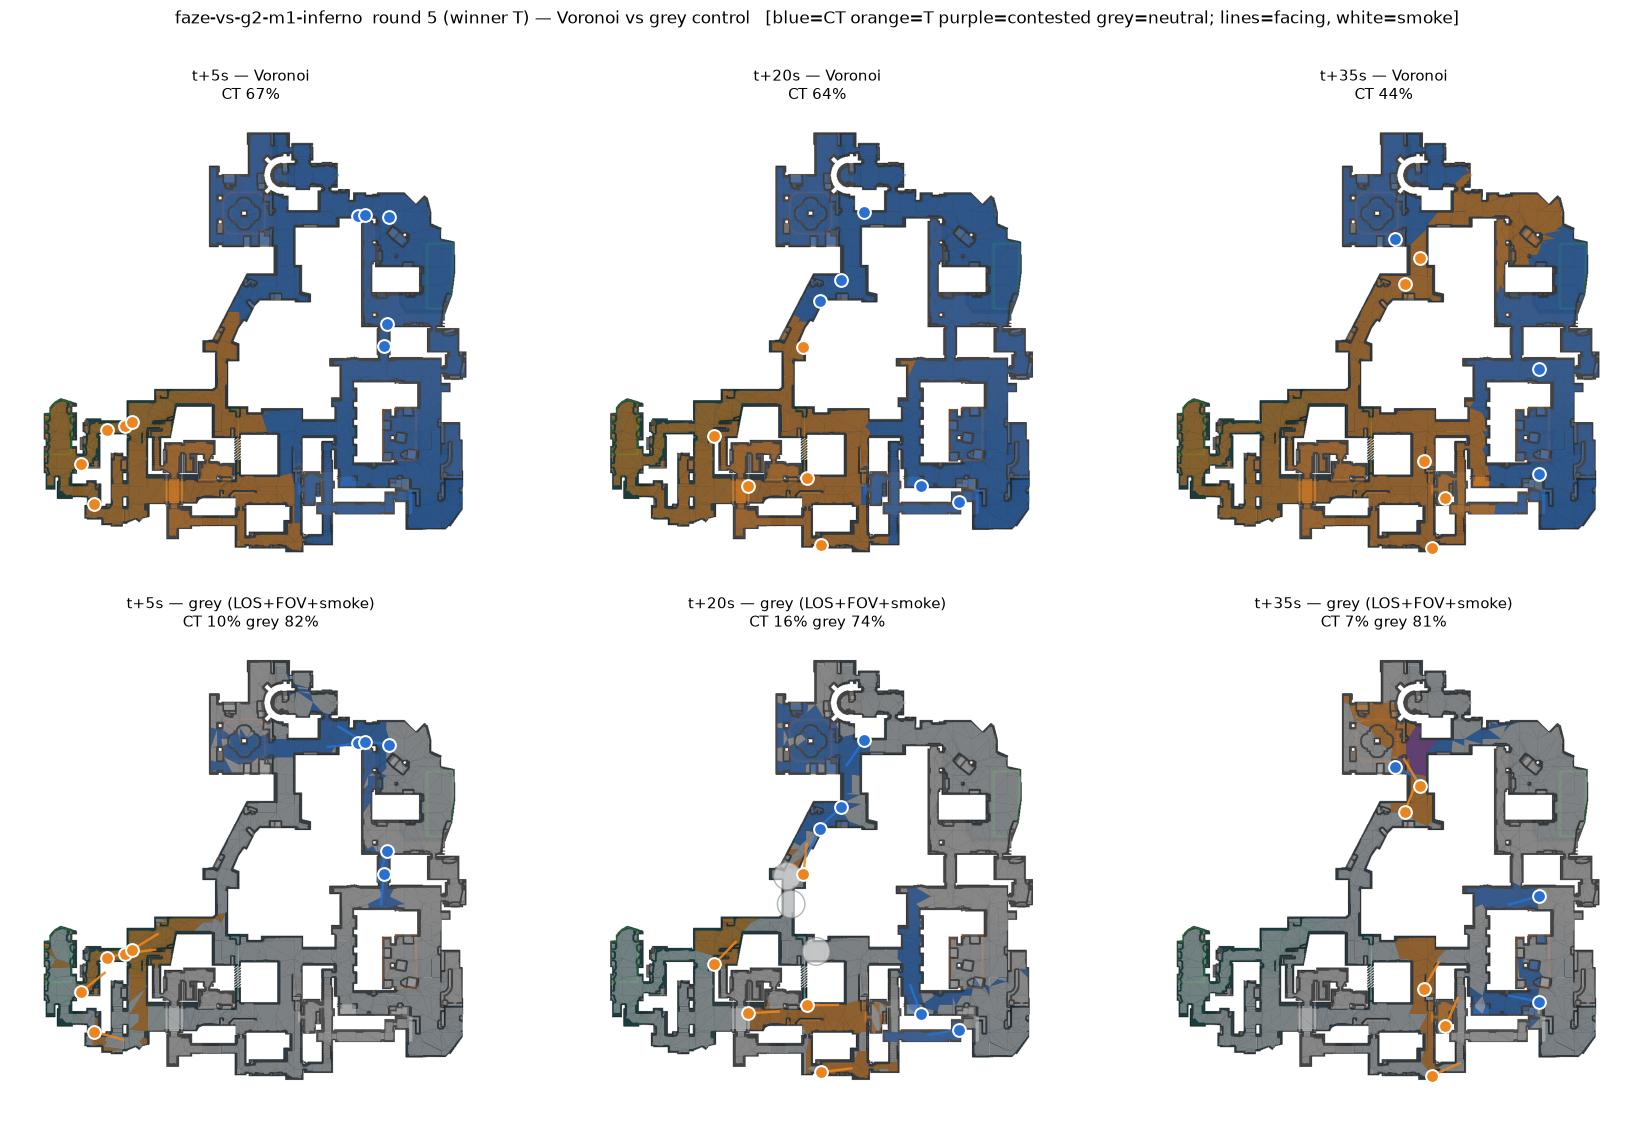
\includegraphics[width=\textwidth]{mapcontrol_compare_faze-vs-g2-m1-inferno_r5.png}
\caption{The same round, three moments, two control models. \textbf{Top:} Voronoi
proximity control partitions the whole map (CT 67\,\%/64\,\%/44\,\%). \textbf{Bottom:}
the LOS+FOV+smoke ``grey'' model, which additionally requires line-of-sight, facing, and
no smoke occlusion --- 74--82\,\% of the map is grey, held by nobody. Blue = CT, orange =
T, purple = contested, grey = neutral; short lines show facing; white discs are smokes.
The bottom row is a far better description of what the players actually control. It is
also the \emph{worse} predictor (Table~\ref{tab:mapcontrol}).}
\label{fig:mapcompare}
\end{figure}

\subsection{Pillar 3 --- Tactical readiness and bomb geometry (42 features)}
\label{sec:pillar3}

Utility inventories (per-type grenade counts per side), AWP presence and the zone the AWP
is in, per-zone player counts for both sides, positional (Shannon) entropy as a measure
of how spread out a side is, and bomb geometry: plant site, plant coordinates, and the
nearest CT's straight-line \emph{and} nav-mesh Dijkstra path distance to the bomb.

The straight-line/path distinction matters more than it sounds. On Inferno a CT can be
10 metres from the bomb through a wall and 30 seconds away through the map.
Figure~\ref{fig:shapdist} shows the consequence: the SHAP dependence for
\texttt{min\_ct\_dist\_to\_bomb} is smooth and monotone-ish, i.e.\ the model treats raw
proximity as a soft signal --- whereas the \emph{path-derived} defuse margin below produces
a hard step. The physics is in the path, not the distance.

\begin{figure}[H]
\centering
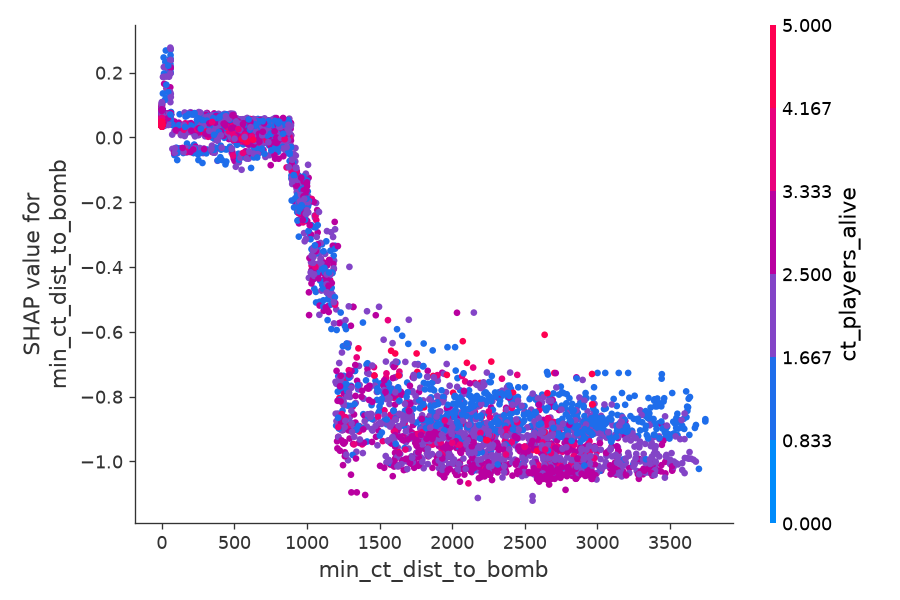
\includegraphics[width=0.62\textwidth]{shap_dependence_min_ct_dist_to_bomb.png}
\caption{SHAP dependence for the nearest CT's straight-line distance to the bomb. A soft,
graded effect --- compare with the sharp feasibility boundary the path-derived defuse
margin produces (Fig.~\ref{fig:shapdefuse}).}
\label{fig:shapdist}
\end{figure}

\paragraph{The defuse race.}
Post-plant, the round stops being a fight and becomes a race against the fuse. We track
the bomb's live state (\emph{carried} / \emph{dropped} / \emph{planted}) from the event
stream, and for each alive CT compute an arrival time (nav path length $\div$ run speed)
plus a defuse duration (5\,s with a kit, 10\,s without). The CT who would actually defuse
is the one with the smallest finish time. Then

\begin{equation}
  \texttt{defuse\_time\_margin}
  \;=\;
  \underbrace{t_{\text{fuse}}}_{\text{time left on bomb}}
  \;-\;
  \Bigl(
    \underbrace{t_{\text{path}}}_{\text{nav path} \,\div\, \text{run speed}}
    \;+\;
    \underbrace{t_{\text{defuse}}}_{5\text{s with kit},\; 10\text{s without}}
  \Bigr),
  \label{eq:defuse}
\end{equation}

which is positive if and only if a defuse is \emph{physically attemptable}. The
zero-crossing is a hard feasibility boundary in the game's physics. A refinement,
\texttt{defuse\_margin\_kit}, computes the margin per CT with that CT's actual kit
status and adds a T-interruption window (how long a T must survive to break the defuse).

\paragraph{Two features we built and rejected.}
We also computed (i) \emph{map control in the neighbourhood of the live bomb} and (ii) a
\emph{dropped-bomb scramble} feature (who is closest to a loose bomb). Both were weak and
redundant. We report them in Sect.~\ref{sec:bomb} rather than quietly dropping them,
because the \emph{reasons} they fail are informative and generalise.

\subsection{Pillar 4 --- Firepower (player skill prior)}
\label{sec:pillar4}

A pre-round skill prior from HLTV per-player statistics, joined on
$(\text{steamid}, \text{year})$ --- keyed by year because skill drifts season to season
and a 2024 rating is not a 2026 rating. We built two versions and report both, because
the progression is part of the finding.

\paragraph{Firepower v1 (9 features).}
Sums of HLTV Rating, ADR and KAST over the players currently alive on each side, plus a
1-v-$N$ clutch score. Simple, dense, and --- as Sect.~\ref{sec:firepower} shows --- almost
entirely a re-encoding of the player count.

\paragraph{Firepower v2 (20 features).}
Built specifically to fix v1's confound. It is \emph{side-aware} (separate CT-side and
T-side Rating, Firepower, Entrying, Trading and Opening statistics, since a player's CT-
and T-side output genuinely differ) and applies \emph{per-player situational gates}: a
lone survivor contributes his Clutching statistic and has Entry/Trading suppressed; a
player with teammates alive contributes Entry and Trading; Opening statistics apply only
when both sides are still 5-alive and an opening duel is actually possible. It adds an
AWP-holder ``sniping'' role flag and a grenade-value-weighted utility term.

\paragraph{Why this pillar is structurally different --- and why that turned out to matter.}
Pillars 1--3 are computed \emph{from the demo itself}: every input is present in the
observation being scored. Pillar~4 is not. It requires an \textbf{external database,
indexed by era}, and is therefore the only pillar that can be \emph{unavailable at
inference time}. In-sample this looks like a minor engineering detail. It is the single
most consequential design decision in the paper (Sect.~\ref{sec:holdout}).

% =====================================================================
\section{Models}
\label{sec:models}

Nine architectures, all evaluated under an identical protocol (Sect.~\ref{sec:protocol}).

\subsection{Classical (5)}
Logistic regression (standardised inputs, L2); random forest (300 trees); XGBoost,
LightGBM and CatBoost.

All three boosters are tuned to \emph{shallow, heavily regularised} trees (depth 3,
$\lambda = 10$, subsample 0.8). \textbf{This matters more than any feature pillar.} Our
initial depth-6 configuration overfit badly; fixing it was worth $+0.007$ AUC --- larger
than the contribution of \emph{any} feature pillar in this paper. We report it as a
warning: a poorly-regularised booster will happily swamp a genuine feature effect, and if
we had run the map-control ablation at depth 6 we would have concluded that map control
does nothing.

\subsection{Deep (3)}
All trained on GPU (NVIDIA B200, PARCC Betty cluster).

\begin{itemize}
  \item \textbf{Causal TCN.} The round is a sequence of per-second feature vectors.
    Dilated causal convolutions (dilations 1/2/4) ensure the prediction at second $t$
    attends only to $t' \le t$: no within-round look-ahead. Sequence-to-sequence, one
    probability per second. This model can in principle learn \emph{momentum}, which the
    per-snapshot models can only see through our hand-built trend and volatility features.
  \item \textbf{Causal Transformer encoder.} Same input, causal self-attention mask,
    sinusoidal positional encodings.
  \item \textbf{GAT (player graph).} The only model that consumes the \emph{raw per-player
    trajectory} --- position, velocity, view angle, health, armour, equipment, kit, side,
    for up to 10 alive players --- rather than aggregates. Masked multi-head self-attention
    over the player set (a graph attention network on the complete player graph),
    permutation-invariant, masked mean-pooled to a round-state embedding. If any
    architecture were going to discover spatial structure our engineered features miss, it
    is this one.
\end{itemize}

\subsection{Ensemble (1)}
Soft-vote (mean predicted probability) over classical and deep members. A logistic
\emph{stack} was also tried and rejected (Sect.~\ref{sec:deep}).

% =====================================================================
\section{Evaluation Protocol}
\label{sec:protocol}

\subsection{Cross-validation}
5-fold \textbf{GroupKFold by match}. We never split a match across folds. Rounds within a
match are strongly correlated --- same players, same tactics, same map side, same day ---
and folding by \emph{round} leaks that correlation across the train/test boundary and
inflates AUC. All in-time numbers in this paper are out-of-fold (OOF) predictions.

\subsection{Metrics}
\begin{description}
  \item[Primary (literature-comparable).] AUC, log-loss, Brier score.
  \item[Complementary.] ECE (10-bin), Brier Skill Score, and \textbf{contested-AUC}: AUC
    restricted to snapshots with equal players alive \emph{and}
    $|\Delta\text{equipment}| \le \$1500$ --- 12.2\,\% of all snapshots.
  \item[Extended.] The Murphy decomposition of the Brier score into
    reliability / resolution / uncertainty; sharpness; calibration slope and intercept
    (bin-free, from a logistic recalibration fit); an adaptive equal-mass ECE and a
    Kolmogorov--Smirnov calibration error (both binning-free, since 10-bin ECE is sensitive
    to bin placement); and a comeback/tail diagnostic (Sect.~\ref{sec:calibration}).
\end{description}

\subsection{Uncertainty}
\textbf{Match-level block bootstrap} ($B = 500$). \emph{Matches}, not snapshots, are the
independent resampling unit; each iteration draws all matches with replacement and
recomputes \emph{every} metric on the fixed OOF predictions. This yields 95\,\% CIs on
AUC, log-loss, Brier, ECE, BSS and contested-AUC alike.

This choice is load-bearing. Treating the $\approx$476k snapshots as independent would
shrink every interval by more than an order of magnitude and make all of our pillar
effects look spuriously decisive --- and would, in particular, have let us claim the deep
models beat the classical ones. They do not (Sect.~\ref{sec:deep}). DeLong's test
corroborates the AUC differences; deep models additionally report a multi-seed mean $\pm$
sd.

\subsection{Out-of-time}
A \textbf{touch-once} 2026 holdout (Sect.~\ref{sec:holdout}). We ran it exactly once. No
model, feature or hyperparameter decision in this paper was made after seeing it. We state
this explicitly because the holdout is the source of our headline claim, and its
evidential value is entirely contingent on that discipline. Any subsequent re-run (e.g.\
after the 2026 skill scrape completes) must be reported as a separate, disclosed
evaluation --- not folded silently into these numbers.

% =====================================================================
\section{Results}
\label{sec:results}

\subsection{The model matrix}
\label{sec:matrix}

Figure~\ref{fig:heatmap} gives the full model $\times$ feature-set grid. In sample, the
best single model is \textbf{logistic regression on all pillars} (EFB2): AUC $0.8519$
(95\,\% CI $0.8451$--$0.8582$). The best overall is the four-model \textbf{soft-vote
ensemble}: $0.8531$ ($0.8460$--$0.8598$), which also has the best calibration (ECE $0.009$,
BSS $0.378$). The economy baseline is $0.8465$. Every pillar's lift is small in pooled AUC
but statistically significant, in the sense that its bootstrap CI excludes zero.

That \emph{logistic regression} wins is itself informative: once the features are built,
the aggregate signal is close to linear, and the non-linear models spend their capacity on
variance rather than bias.

\begin{figure}[H]
\centering
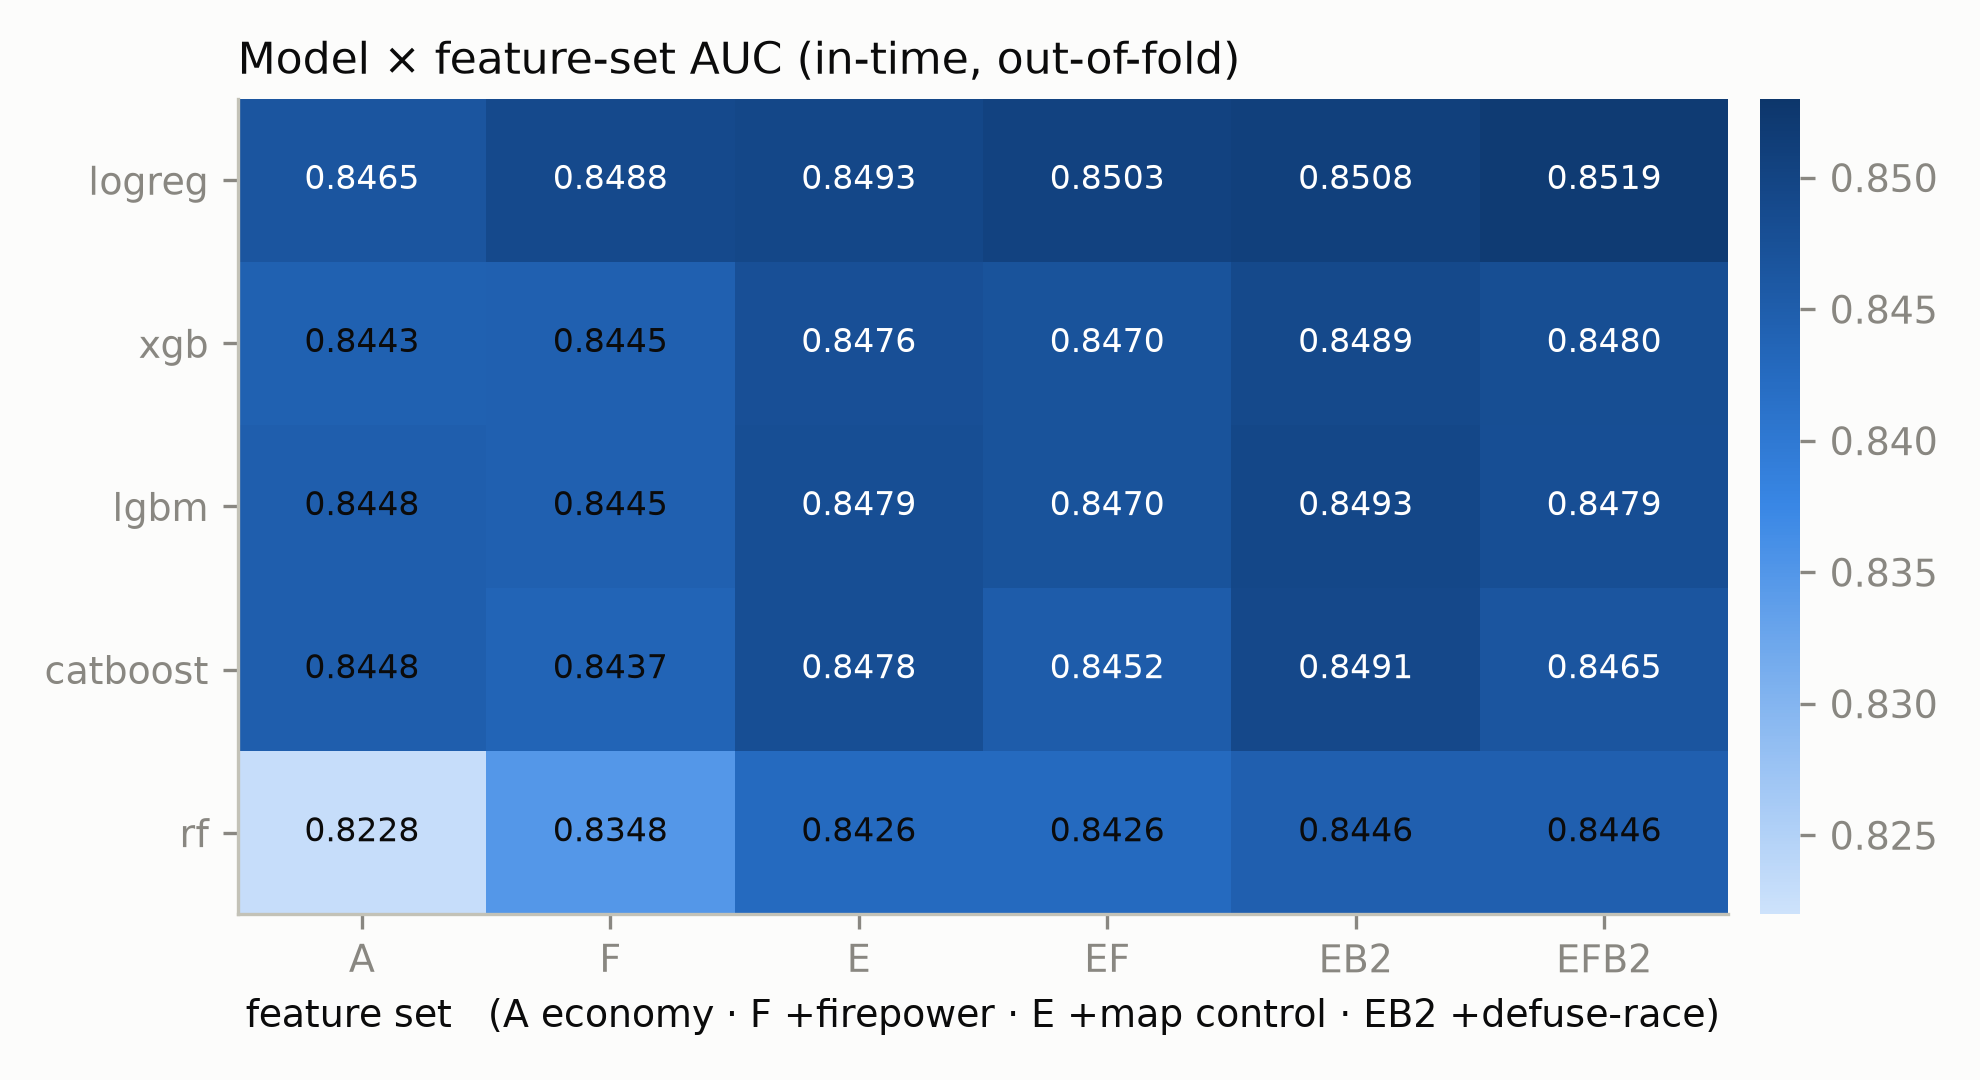
\includegraphics[width=0.8\textwidth]{F3_heatmap.png}
\caption{Model $\times$ feature-set AUC (in-time, out-of-fold). The grid is strikingly
flat: the spread across nine architectures is smaller than the spread across feature sets,
and both are small.}
\label{fig:heatmap}
\end{figure}

\subsection{Where the signal actually lives: contested-AUC}
\label{sec:contested}

Pooled AUC hides the model's real behaviour. Conditioning on how \emph{even} the round is:

\begin{table}[H]
\centering
\caption{AUC by round subset (XGBoost, out-of-fold).}
\label{tab:contested}
\begin{tabular}{lrrr}
\toprule
Subset & Share of snapshots & A (economy) & EB2 \\
\midrule
All snapshots             & 100\,\%           & 0.844 & 0.849 \\
Equal players alive       & 52\,\%            & 0.705 & 0.711 \\
Even economy              & ---               & 0.683 & 0.689 \\
\textbf{Contested (both)} & \textbf{12.2\,\%} & \textbf{0.580} & \textbf{0.586} \\
\bottomrule
\end{tabular}
\end{table}

\begin{figure}[H]
\centering
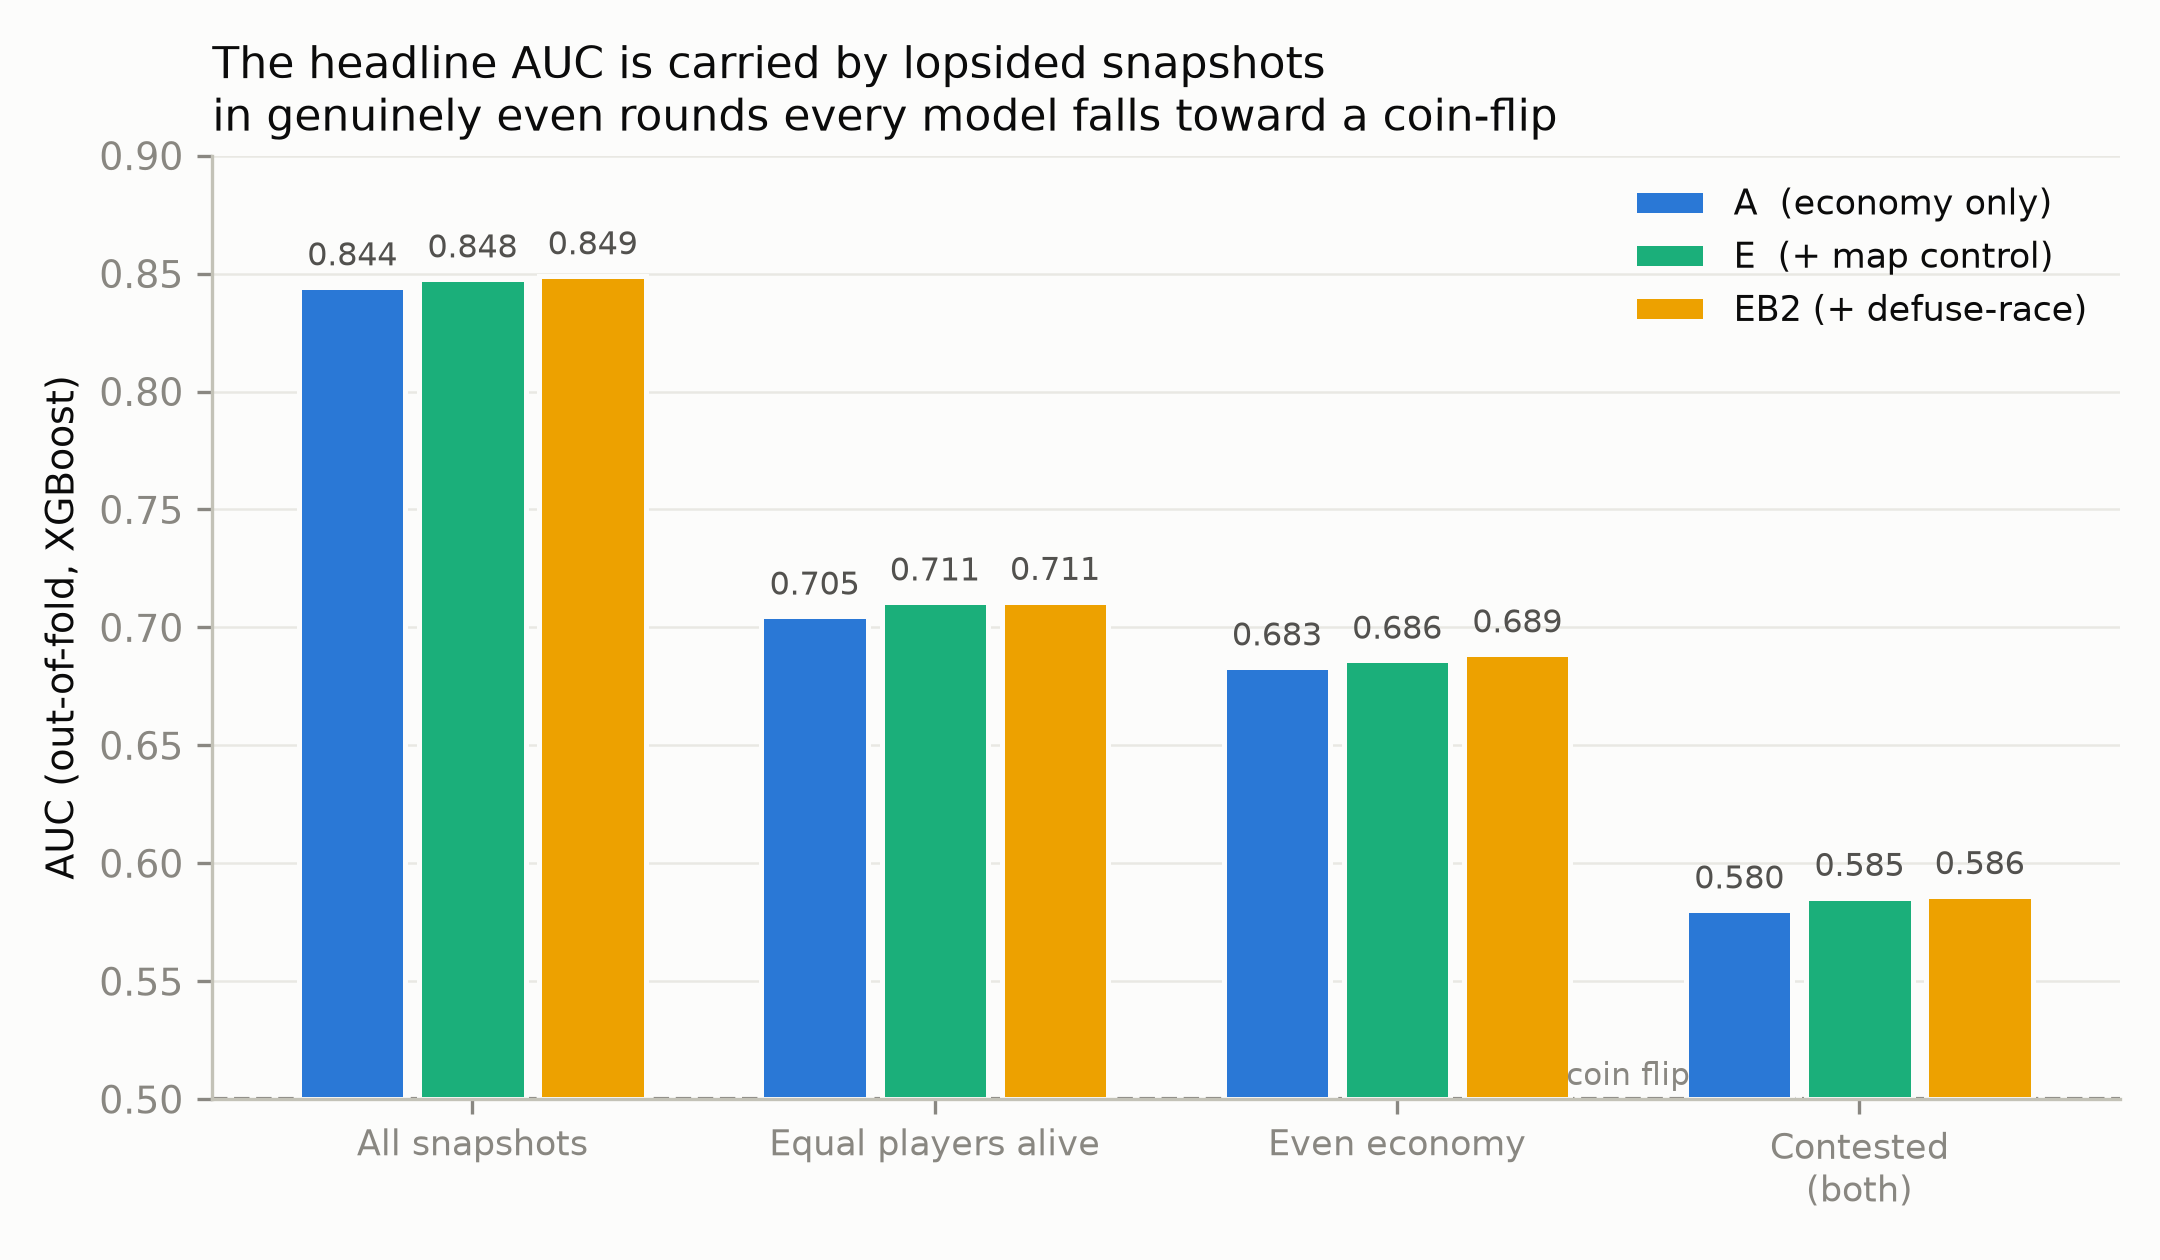
\includegraphics[width=0.95\textwidth]{F2_collapse.png}
\caption{The headline AUC is carried by lopsided snapshots; in genuinely even rounds every
model falls toward a coin flip.}
\label{fig:collapse}
\end{figure}

\textbf{The economy baseline collapses from $0.844$ to $0.580$ --- barely above a coin
flip.} The headline number is carried by lopsided snapshots (5-v-2, eco vs full-buy) that
any model gets right, and which dominate per-second data precisely because a lopsided round
\emph{stays} lopsided for many consecutive seconds. In the states a viewer actually cares
about --- the round is even, the outcome is genuinely live --- \emph{no model in this study
exceeds $0.60$}.

We regard this as the honest characterisation of the state of the art. It does not mean the
models are useless: correctly saying ``this 5-v-2 is over'' is what a broadcast overlay
spends most of its time doing. It means the number conventionally reported is close to a
measure of \emph{how often the game is lopsided}, and reporting it alone invites the reader
to over-estimate what the model knows.

The spatial pillars provide a consistent lift throughout, slightly larger in the contested
regime. Their aggregate contribution is modest ($\approx +0.003$--$0.005$ AUC) but robust:
significant across all five classical architectures. \emph{We resist the temptation} to
claim the spatial features are \emph{especially} valuable in contested rounds --- the
contested lift ($+0.006$) is not reliably larger than the pooled lift ($+0.005$). The honest
statement is that the pillars help uniformly while the \emph{baseline} collapses.

\subsection{Map control: realistic $\ne$ predictive (unless stabilised)}
\label{sec:mapcontrol}

This is the central spatial result. Recall Fig.~\ref{fig:mapcompare}: the grey model is
visibly the truer description of the game. Here is what it buys us.

\begin{table}[H]
\centering
\caption{The map-control ablation (XGBoost, out-of-fold). The most physically faithful
representation is the least predictive.}
\label{tab:mapcontrol}
\begin{tabular}{lrl}
\toprule
Representation & AUC & Verdict \\
\midrule
Economy only (A)                  & 0.8443 & baseline \\
\textbf{+ Voronoi (proximity)}    & \textbf{0.8468} & best single control model \\
+ Grey (LOS + FOV + smoke)        & 0.8451 & \emph{most faithful, least predictive} \\
+ Territory (grey + 15\,s memory) & 0.8453 & memory restores it \\
\bottomrule
\end{tabular}
\end{table}

The instantaneous LOS/FOV/smoke model is a far better description of what the players can
actually \emph{see and contest} --- and it is a \textbf{worse} predictor than naive
proximity.

The reason is temporal. Yaw is twitchy: a player flicks his crosshair across 90 degrees in
a fraction of a second, and the set of areas he ``controls'' under an instantaneous FOV test
churns violently from tick to tick. Instantaneous control therefore \emph{flickers}, while
round outcomes depend on \emph{stable} territorial state --- who has \emph{taken} banana, not
who happens to be looking down it at this exact instant. Granting the same model a 15-second
memory (cleared space stays yours until contested) recovers parity with Voronoi.

\begin{quote}
\textbf{Predictiveness comes from temporal stability, not physical fidelity.}
\end{quote}

This carries a concrete methodological warning. A practitioner who builds a vision-based
control surface, finds it does not beat a proximity baseline, and concludes that ``map
control does not predict outcomes'' has drawn the wrong conclusion from the right
experiment. The representation was too jittery; the concept was fine.

Voronoi and territory are largely redundant with one another ($r = 0.47$); stacking
territory on top of Voronoi yields $\approx 0$ additional AUC. We therefore retain Voronoi
as the primary control feature --- the crude model, kept for the un-crude reason that it is
stable.

\paragraph{What the lift looks like in a single round.}
Aggregate AUC deltas of $+0.003$ are easy to dismiss, so Fig.~\ref{fig:controlshift} shows
a round where the map-control pillar is doing something a human analyst would recognise. The
economy-only model (grey) finishes the round convinced the CTs are winning --- it spikes to
$0.82$ --- because on paper the CTs have the equipment. The map-control model (red) sees that
the T side has actually taken the map and holds its prediction near $0.28$, a $-54$
percentage-point correction. The T side won.

\begin{figure}[H]
\centering
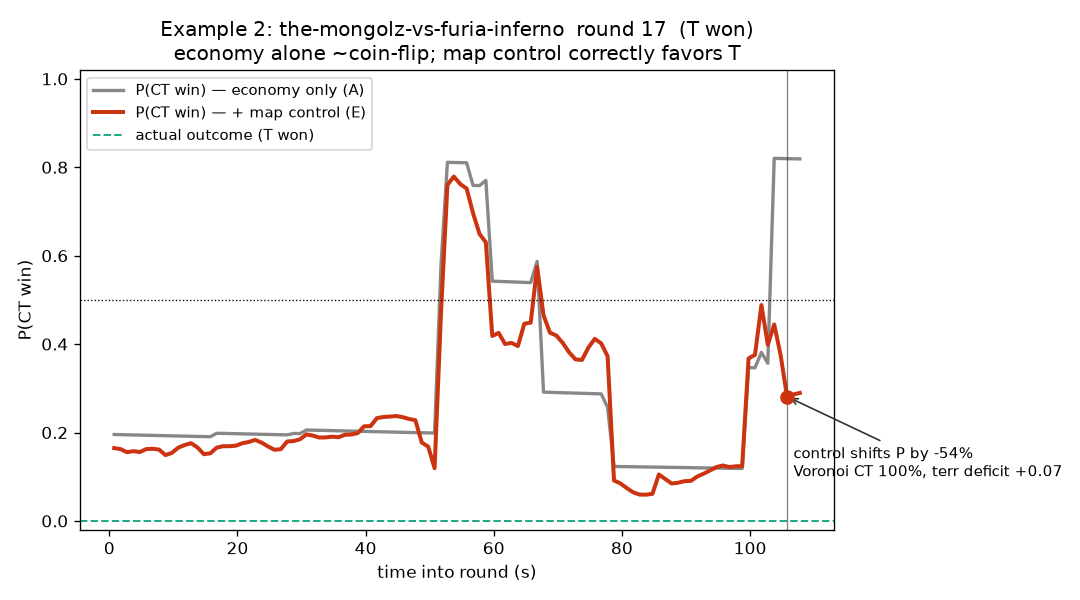
\includegraphics[width=0.9\textwidth]{control_shift_example_2_the-mongolz-vs-furia-inferno_r17.png}
\caption{A round where map control earns its keep. Economy alone (grey) ends up near
$0.82$ for the CTs; adding map control (red) corrects this to $\approx 0.28$. The T side
won. These corrections are individually large but rare, which is exactly why the pooled AUC
lift is small.}
\label{fig:controlshift}
\end{figure}

That last point deserves emphasis, because it is a general property of this problem:
\emph{large, correct, individually convincing corrections that are nonetheless rare produce
small pooled AUC gains.} This is another reason the pooled number is a poor lens.

\subsection{Bomb geometry: the defuse race}
\label{sec:bomb}

\texttt{defuse\_time\_margin} (Eq.~\ref{eq:defuse}) is \textbf{permutation-importance rank
\#8 of 68} --- the strongest single feature added after economy. Adding the bomb-live pillar
(set EB2) is significant on \emph{every} architecture (all bootstrap CIs exclude zero), and
the gain is concentrated exactly where the physics says it should be:

\begin{itemize}
  \item \textbf{post-plant log-loss falls 7--8\,\%} (XGBoost: $0.187 \to 0.172$; post-plant
    AUC $0.962 \to 0.967$);
  \item \textbf{endgame log-loss} falls across all models ($0.401 \to 0.396$);
  \item \textbf{calibration is preserved} (ECE $\approx 0.013$): the feature adds
    discrimination without distorting the probabilities.
\end{itemize}

Figure~\ref{fig:shapdefuse} shows the mechanism, and it is the cleanest single piece of
evidence in the paper. The SHAP contribution is a \textbf{step function with its jump at
exactly zero} --- the feasibility boundary. When the margin is positive (a defuse is
physically attemptable) the feature contributes $\approx 0$; the instant it goes negative,
the contribution drops to $\approx -0.8$ and stays there. The model has learned the game's
physics as a hard constraint: \emph{when a defuse becomes impossible, abandon the CTs}.

Contrast this with the smooth, graded SHAP curve for raw distance-to-bomb
(Fig.~\ref{fig:shapdist}). Same underlying geometry; one encoding makes the boundary
learnable and the other does not. \textbf{This is the whole argument for
physically-derived features in one pair of plots}, and it is behaviour none of the deep
models discovered on their own from the raw distances.

\begin{figure}[H]
\centering
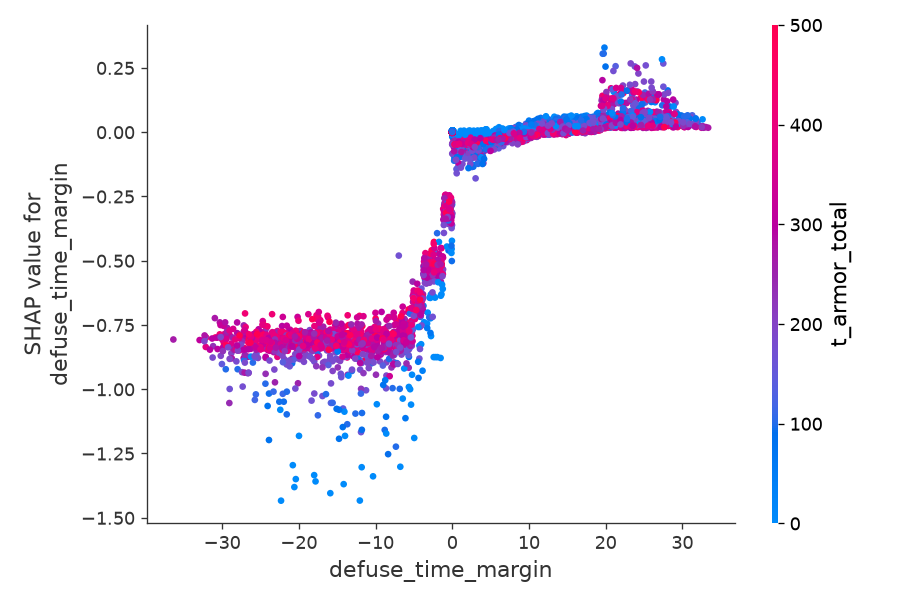
\includegraphics[width=0.62\textwidth]{shap_dependence_defuse_time_margin.png}
\caption{SHAP dependence for \texttt{defuse\_time\_margin}. The step at zero is the
\emph{feasibility boundary}: to the right a defuse is physically attemptable and the
feature is near-neutral; to the left it is impossible and the model confidently writes the
CTs off. The model has learned a hard physical constraint, not a soft correlation.}
\label{fig:shapdefuse}
\end{figure}

\paragraph{Negative results, reported.}
Neither \emph{map control around the live bomb} nor the \emph{dropped-bomb scramble} feature
helped; both were weak and redundant. The reasons generalise:

\begin{itemize}
  \item A loose (dropped) bomb is a \emph{consequence} of a losing round, not a cause of one.
    The T carrying it died --- and ``a T died'' is already in the model. The feature is
    downstream of information we already have.
  \item Bomb-neighbourhood ownership duplicates the existing site-control features, because
    the bomb is nearly always at a site.
\end{itemize}

The lesson is that what matters post-plant is the \emph{race geometry} of
Eq.~\ref{eq:defuse}, not local ownership of the ground the bomb happens to sit on.

\subsection{Firepower: anatomy of a confound}
\label{sec:firepower}

Firepower is the weakest of the four pillars in-sample, and the most instructive.

\paragraph{v1, and the most seductive artifact in the study.}
The v1 feature $\texttt{ct\_rating\_sum} - \texttt{t\_rating\_sum}$ came out at
\textbf{permutation-importance rank \#1} of all 68 features. Taken at face value this is a
triumph for the skill pillar: player quality is the single most important thing in
Counter-Strike, exactly as folklore says.

It is nothing of the sort, and Fig.~\ref{fig:shapfirepower} shows why in one glance. The
feature's values \textbf{cluster at the integers 0, 1, 2, 3, 4, 5}. It is not measuring
skill; it is \emph{counting players}. Because rating is \emph{summed over alive players} and
professional ratings live in a narrow band around 1.0, the sum is dominated by how many
terms are in it. The correlation with the plain player-count advantage is \textbf{0.987}, and
the two predict the outcome identically ($r = 0.498$ each).

\begin{figure}[H]
\centering
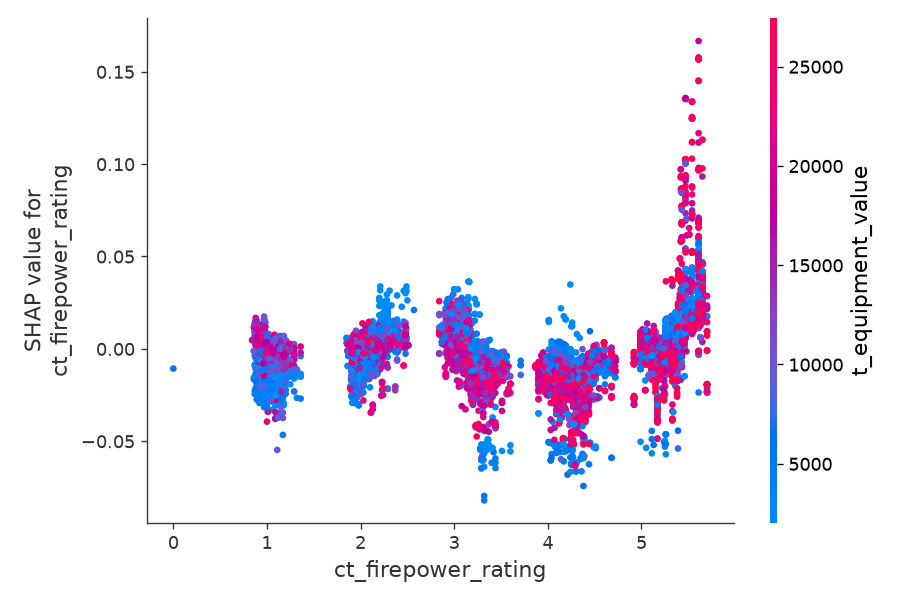
\includegraphics[width=0.62\textwidth]{shap_dependence_ct_firepower_rating.png}
\caption{The count confound, made visible. The ``team firepower rating'' is a \emph{sum} of
per-player ratings over alive players, and professional ratings cluster near 1.0 --- so the
feature's values pile up at the integers 0--5. The top-ranked ``skill'' feature is mostly a
re-encoding of \emph{how many players are alive}, which the economy pillar already supplies.
Its \emph{marginal} contribution is $\approx 0$.}
\label{fig:shapfirepower}
\end{figure}

This is a cautionary tale about permutation importance on collinear features: it will rank a
proxy above the thing it proxies for, and it will do so confidently.

\paragraph{v2, which half-works.}
v2 (Sect.~\ref{sec:pillar4}) was built to fix this. It partially does: it helps the linear
model (logistic contested-AUC $0.593 \to 0.603$; logistic EFB2 $0.8515 \to 0.8519$, the best
single model in the study). But it \emph{hurts} the tree models. Twenty sparse,
situationally-gated, frequently-\texttt{NaN} features are exactly what a gradient-boosted
model overfits: EF $<$ E on every booster, significantly so on CatBoost ($-0.0026$). And
because v2 kept the \emph{sums}, the count confound survives.

\paragraph{Summary.}
F$-$A is significant only on logistic regression ($+0.0022$, CI $0.0003$--$0.0045$); on
XGBoost, LightGBM and CatBoost the CI includes zero. Adding firepower on top of the other
pillars (EF$-$E) is $\approx 0$ everywhere. We considered a per-capita re-encoding (mean
rather than sum) to break the confound and did not pursue it --- because
Sect.~\ref{sec:holdout} revealed that the pillar's \emph{binding} constraint is not its
encoding at all.

\subsection{What the models actually use}
\label{sec:importance}

Figure~\ref{fig:permimp} shows collinearity-robust permutation importance for set E across
all five classical models. Two things are worth noting.

First, the top of the table is \textbf{economy}: equipment value and health for both sides,
across every model. This is the honest picture --- and it is consistent with the
contested-AUC collapse (Sect.~\ref{sec:contested}), since equipment and health are precisely
the variables that go to zero in a lopsided round.

Second, look at \texttt{min\_ct\_dist\_to\_bomb}: it is the single largest feature for
\emph{logistic regression} (blue) and comparatively minor for the tree models. This is a
useful reminder that ``feature importance'' is a property of the \emph{model}, not of the
world. The linear model leans hard on a monotone spatial feature because it cannot represent
the interaction the trees construct instead.

\begin{figure}[H]
\centering
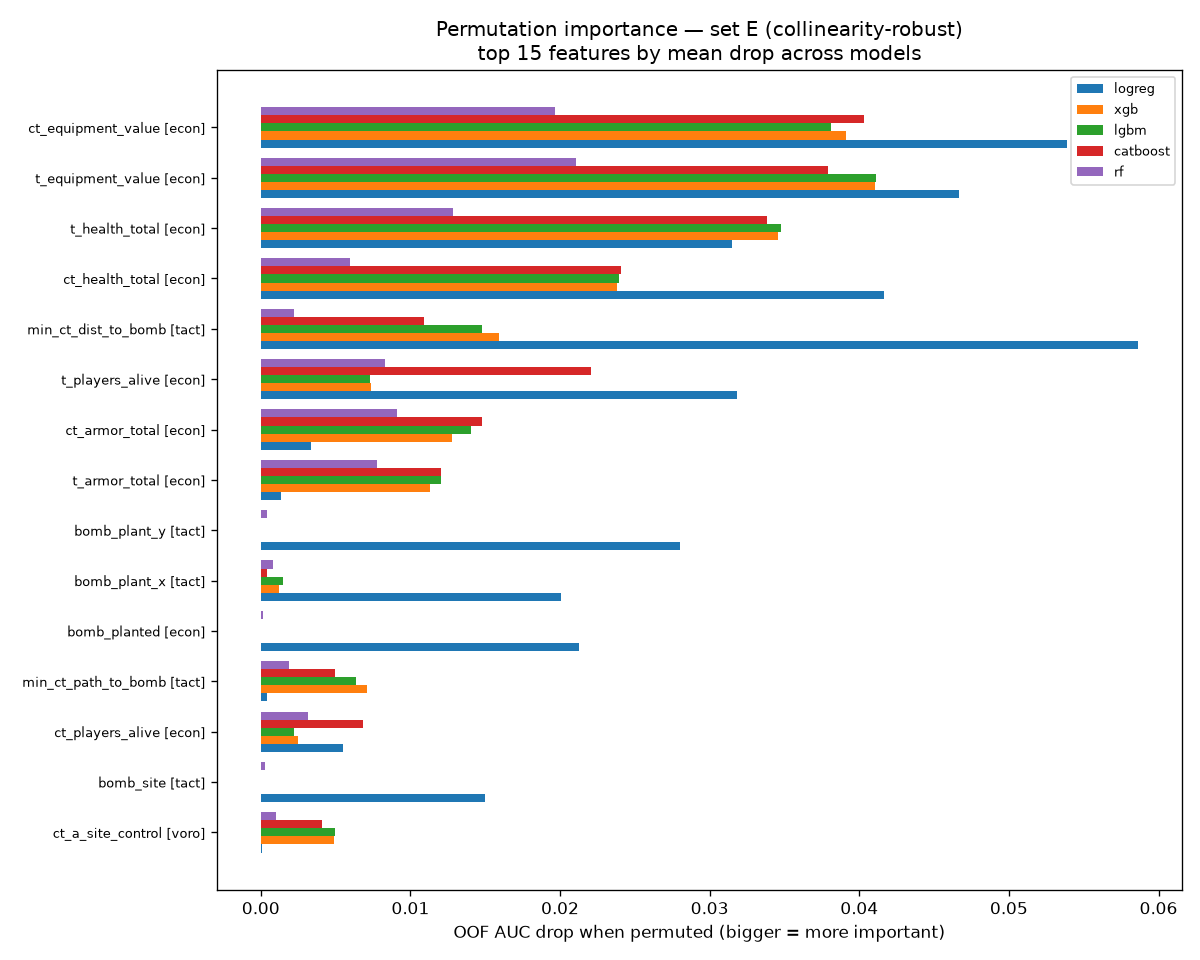
\includegraphics[width=0.92\textwidth]{permutation_importance_E.png}
\caption{Permutation importance (OOF AUC drop when a feature is shuffled), set E, all five
classical models. Economy dominates. Note that \texttt{min\_ct\_dist\_to\_bomb} is the top
feature for logistic regression but minor for the trees: importance is a property of the
model, not of the game.}
\label{fig:permimp}
\end{figure}

\subsection{Deep models: a statistical dead heat}
\label{sec:deep}

\begin{table}[H]
\centering
\caption{Neither the sequence models nor the graph model beats a calibrated logistic
regression. All intervals overlap all point estimates.}
\label{tab:deep}
\begin{tabular}{lrl}
\toprule
Model & AUC & 95\,\% CI \\
\midrule
Ensemble (soft-vote)             & 0.8531 & (0.8460, 0.8598) \\
Logistic regression (EFB2)       & 0.8519 & (0.8451, 0.8582) \\
LightGBM (EB2)                   & 0.8493 & (0.8424, 0.8558) \\
TCN (causal, sequence)           & 0.8488 & (0.8420, 0.8557) \\
Transformer (causal)             & 0.8473 & (0.8398, 0.8541) \\
GAT (raw player trajectories)    & 0.8465 & (0.8396, 0.8534) \\
\bottomrule
\end{tabular}
\end{table}

\begin{figure}[H]
\centering
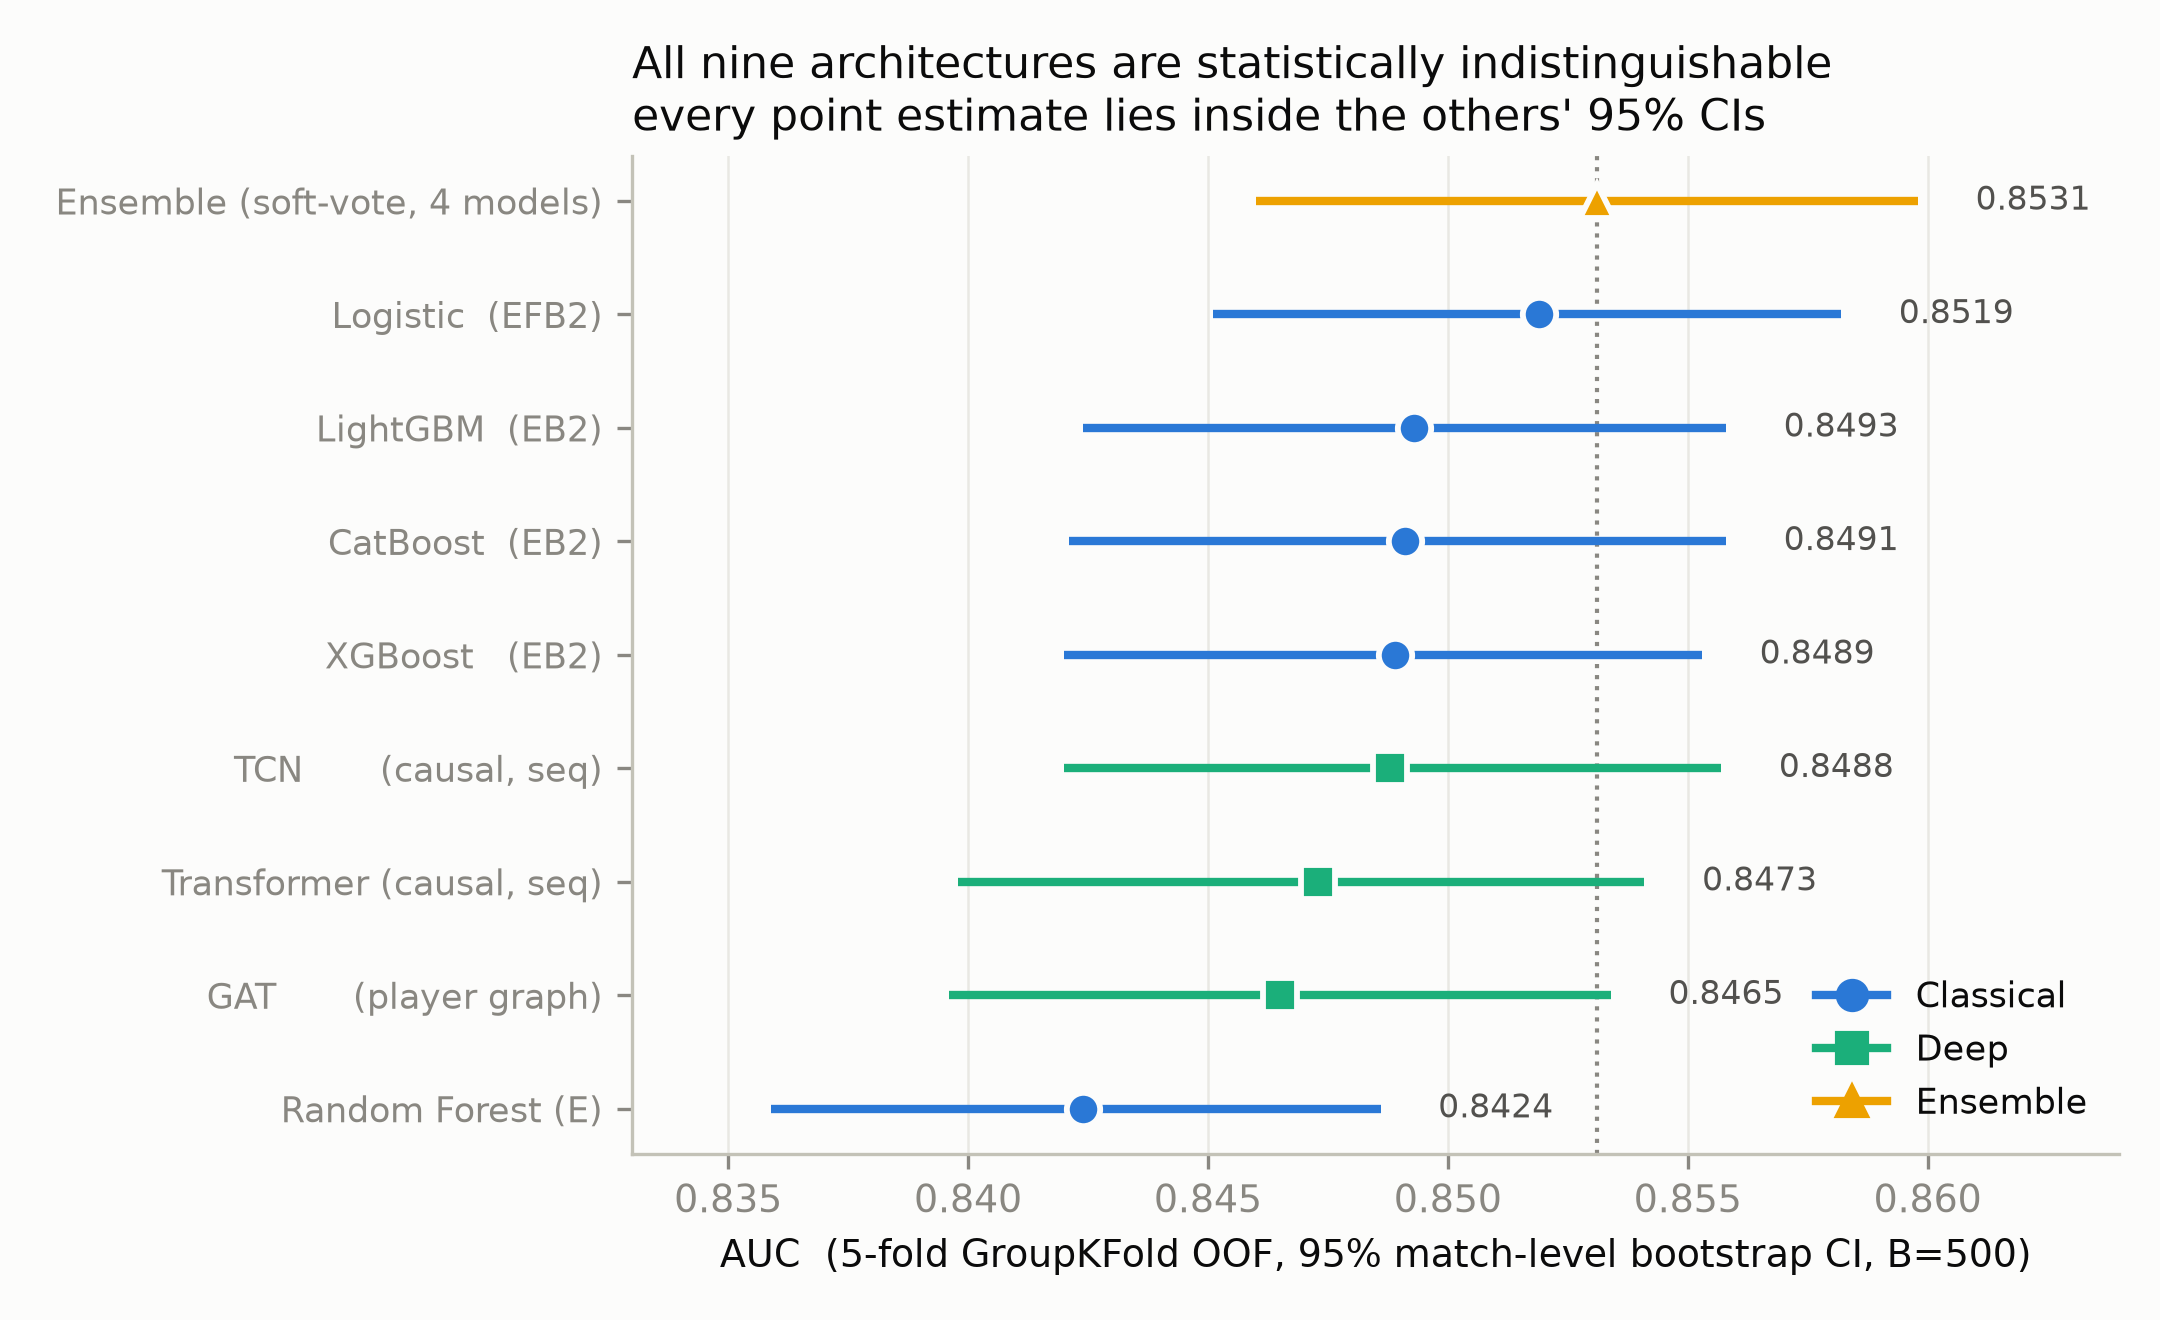
\includegraphics[width=0.95\textwidth]{F1_forest.png}
\caption{All nine architectures with 95\,\% match-level bootstrap CIs. Every point estimate
lies inside the others' intervals.}
\label{fig:forest}
\end{figure}

\textbf{Every point estimate lies inside the others' 95\,\% confidence intervals.} Neither
the sequence models --- which can see \emph{momentum} --- nor the graph model --- which sees
the raw positions, velocities and view angles our aggregates throw away --- beats a
calibrated logistic regression.

Three observations sharpen this.

\begin{enumerate}
  \item \textbf{Sequence length is critical} for the TCN: AUC $0.849$ at 160 timesteps,
    $0.826$ at 100, $0.780$ at 64. Truncation discards the decisive late-round snapshots. A
    reader seeing only the 64-step number would wrongly conclude sequence models are
    hopeless here --- and an author in a hurry might have published exactly that.
  \item \textbf{Multi-seed variance is tiny} ($0.8485 \pm 0.0004$). The tie is not an
    artifact of an unlucky initialisation.
  \item \textbf{The deep models still earn their place in the ensemble.} The soft-vote of
    classical + deep beats either family alone --- the textbook diversity benefit. A logistic
    \emph{stack} matched the soft-vote's AUC but destroyed calibration (ECE $0.042$) and was
    rejected: for a live win-probability product a well-discriminating but badly-calibrated
    model is worse than useless, because the number on screen \emph{is} the product.
\end{enumerate}

\paragraph{Interpretation.}
The engineered features already encode what these architectures would otherwise have to
learn --- trend and volatility for the TCN, zone control for the GAT --- and 220 matches
($\approx 4{,}900$ rounds) is a small corpus for a neural network. This is a statement about
\emph{this data scale}, not a claim that deep learning cannot help. We would expect the GAT
in particular to pull ahead given an order of magnitude more matches, precisely because it is
the only model with access to information the feature engineering discards.

\subsection{Honest probabilities: calibration, phases, and comebacks}
\label{sec:calibration}

A win-probability model's output \emph{is} the product. Discrimination is necessary;
calibration is what makes the number mean anything.

Figure~\ref{fig:reliability} is the reliability diagram with bootstrap CIs. Both the linear
and the tree model sit on the diagonal within error nearly everywhere (logreg EFB2 ECE
$0.016$, CI $0.013$--$0.023$; xgb EFB2 ECE $0.013$, CI $0.010$--$0.020$). The Murphy
decomposition shows the gain from adding pillars is \emph{resolution} (discrimination), not
reliability: the features add skill \emph{without} costing calibration --- an outcome one
wants and is not guaranteed.

\begin{figure}[H]
\centering
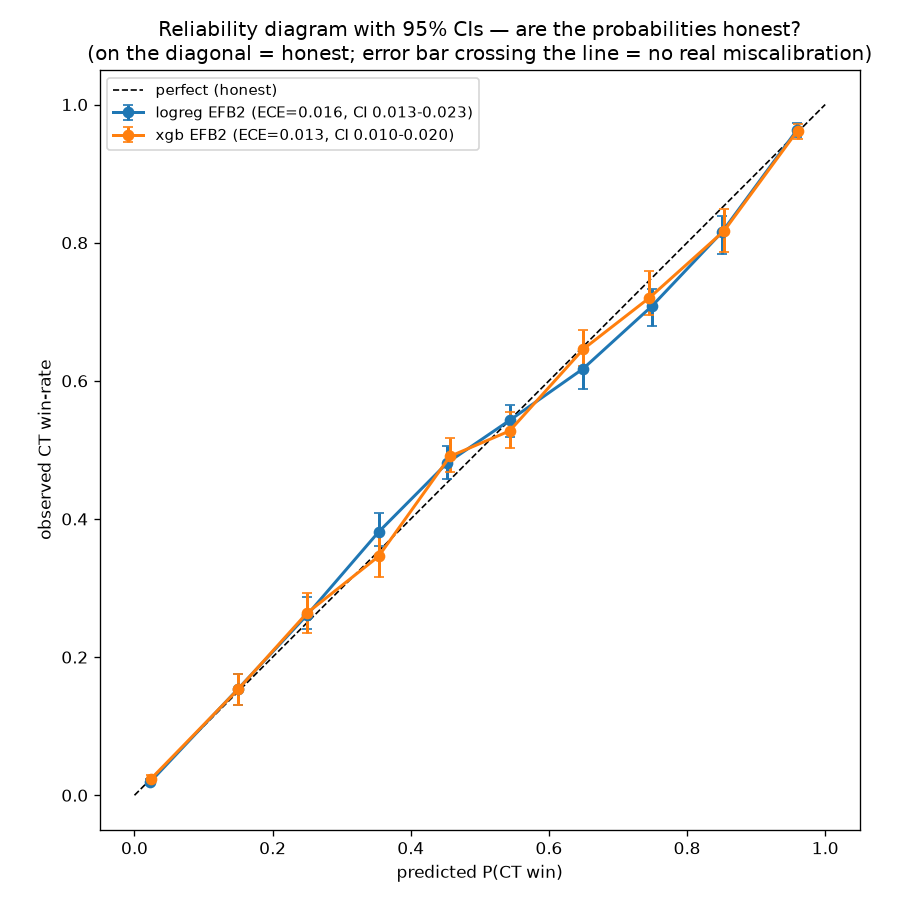
\includegraphics[width=0.6\textwidth]{calibration.png}
\caption{Reliability with 95\,\% bootstrap CIs. Error bars crossing the diagonal indicate no
real miscalibration. Both models are honest.}
\label{fig:reliability}
\end{figure}

Aggregate ECE can hide a model that is honest on average and dishonest at a particular phase
of the round, so Fig.~\ref{fig:caltime} breaks calibration out by time into the round. Both
models stay near or below the $0.02$ ``well-calibrated'' line throughout, and both are
\emph{best} at the end ($30\text{s}+$) --- reassuring, since that is when the model is most
confident and most consequential. The linear model is slightly worse mid-round (25--30\,s),
which is where tactical situations are most complex and least linear.

\begin{figure}[H]
\centering
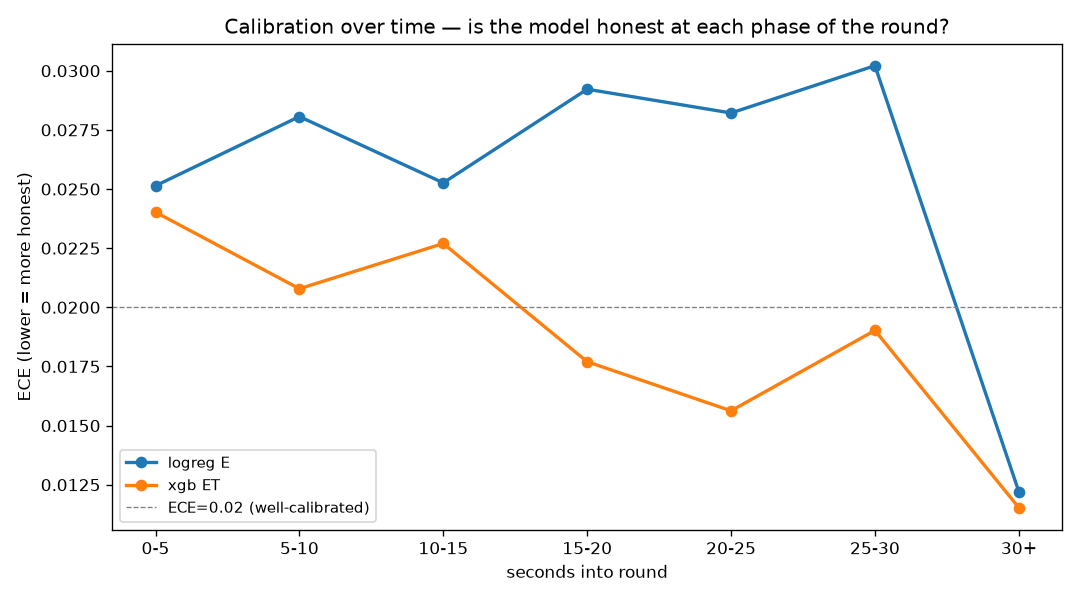
\includegraphics[width=0.8\textwidth]{calibration_over_time.png}
\caption{Calibration by phase of round. Both models are honest at every phase, and most
honest at the end.}
\label{fig:caltime}
\end{figure}

\paragraph{The comeback/tail diagnostic.}
Standard metrics say nothing about whether a live model's \emph{write-offs} are trustworthy
--- and a write-off is the most consequential thing a broadcast overlay says. On the tails:
when the model says 5\,\%, the side wins $0.7\,\%$ of the time; when it says 10\,\%, it wins
$6.8\,\%$. The eventual winner was written off ($\le 10\,\%$) at some moment in
\textbf{7.2\,\% of rounds}, and those calls are calibrated. A viewer who watches the curve
dip to 10\,\% and sees a comeback roughly one time in fourteen is seeing an honest number.

\subsection{What the model looks like live}
\label{sec:live}

Figure~\ref{fig:winprob} is the actual deliverable: a per-second win-probability curve with a
bootstrap uncertainty band, kills and the bomb plant marked.

It repays study, because it shows both the model's competence and its limits. The curve is
\emph{step-like}: it is essentially flat between kills and jumps at them. The model is, to a
first approximation, a kill-counter with a good sense of what each kill is worth in context
--- which is a fair description of what economy-plus-state features can be. And the
uncertainty band is \emph{wide} (mean width $0.21$): the model knows it does not know. Note
the plant at $t = 55$s pushes P(CT win) down to $0.25$ and holds it there, flat, for twenty
seconds --- the defuse-race feature keeping the CTs written off until a late kill re-opens
the round.

\begin{figure}[H]
\centering
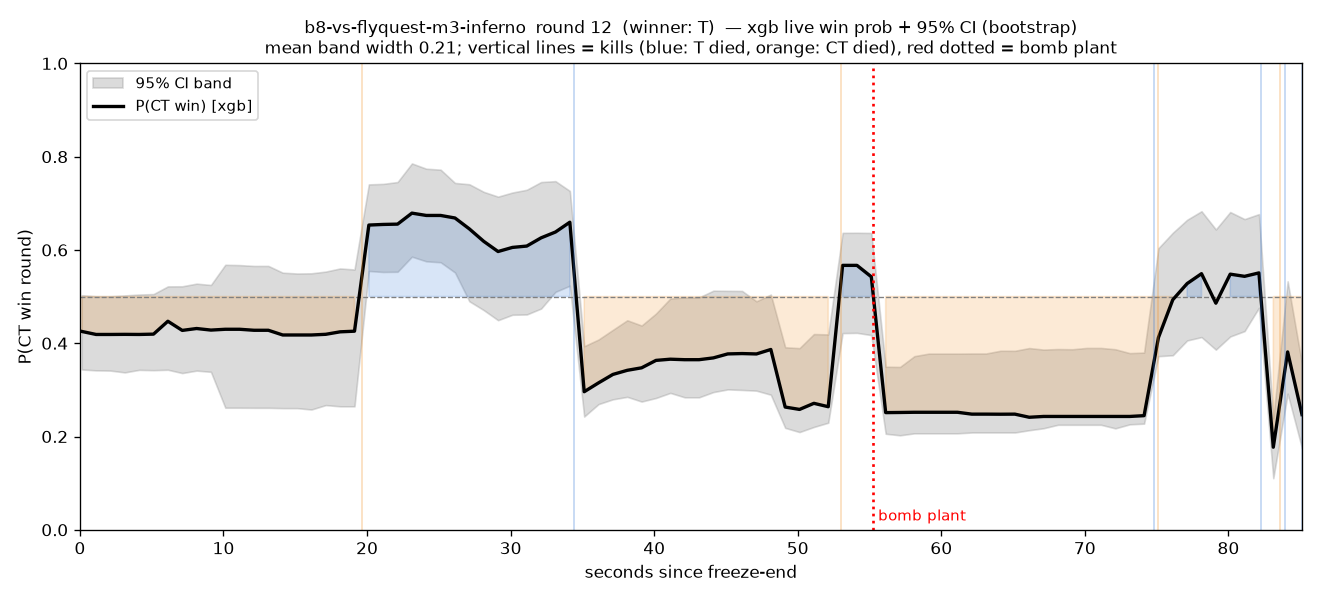
\includegraphics[width=\textwidth]{winprob_b8-vs-flyquest-m3-inferno_r12_xgb.png}
\caption{A live win-probability curve with 95\,\% bootstrap band. Vertical lines are kills
(blue: a T died; orange: a CT died); the red dotted line is the bomb plant. The curve is
step-like --- flat between kills, jumping at them --- and the band is wide (mean $0.21$). Both
are honest reflections of what this model does and does not know.}
\label{fig:winprob}
\end{figure}

\subsection{The out-of-time holdout: the model transfers, its skill prior does not}
\label{sec:holdout}

We trained each model on the full 220-match set (2024--25) and evaluated \textbf{once} on the
27 unseen 2026 matches.

\begin{table}[H]
\centering
\caption{In-time (out-of-fold) vs.\ out-of-time (2026) AUC.}
\label{tab:holdout}
\begin{tabular}{llrrr}
\toprule
Set & Model & In-time & Out-of-time & $\Delta$ \\
\midrule
\textbf{EB2}  & LightGBM      & 0.8493 & \textbf{0.8501} & $+0.0008$ \\
EB2           & XGBoost       & 0.8489 & 0.8497          & $+0.0007$ \\
E             & XGBoost       & 0.8476 & 0.8476          & $\phantom{+}0.0000$ \\
\midrule
\textbf{EFB2} & Logistic reg. & \textbf{0.8519} & \textbf{0.8236} & $\mathbf{-0.0283}$ \\
EFB2          & Random forest & 0.8446 & 0.8159          & $-0.0287$ \\
EFB2          & LightGBM      & ---    & ---             & $-0.0155$ \\
EFB2          & XGBoost       & ---    & ---             & $-0.0136$ \\
\bottomrule
\end{tabular}
\end{table}

Figure~\ref{fig:holdout} is the result in one picture. Points on the diagonal did not degrade.
\textbf{Every non-firepower configuration (blue, orange, green) sits on or above the line.}
\textbf{Every firepower configuration (red diamonds) falls below it}, and the further a
firepower model was ahead in-sample, the further it falls.

\begin{figure}[H]
\centering
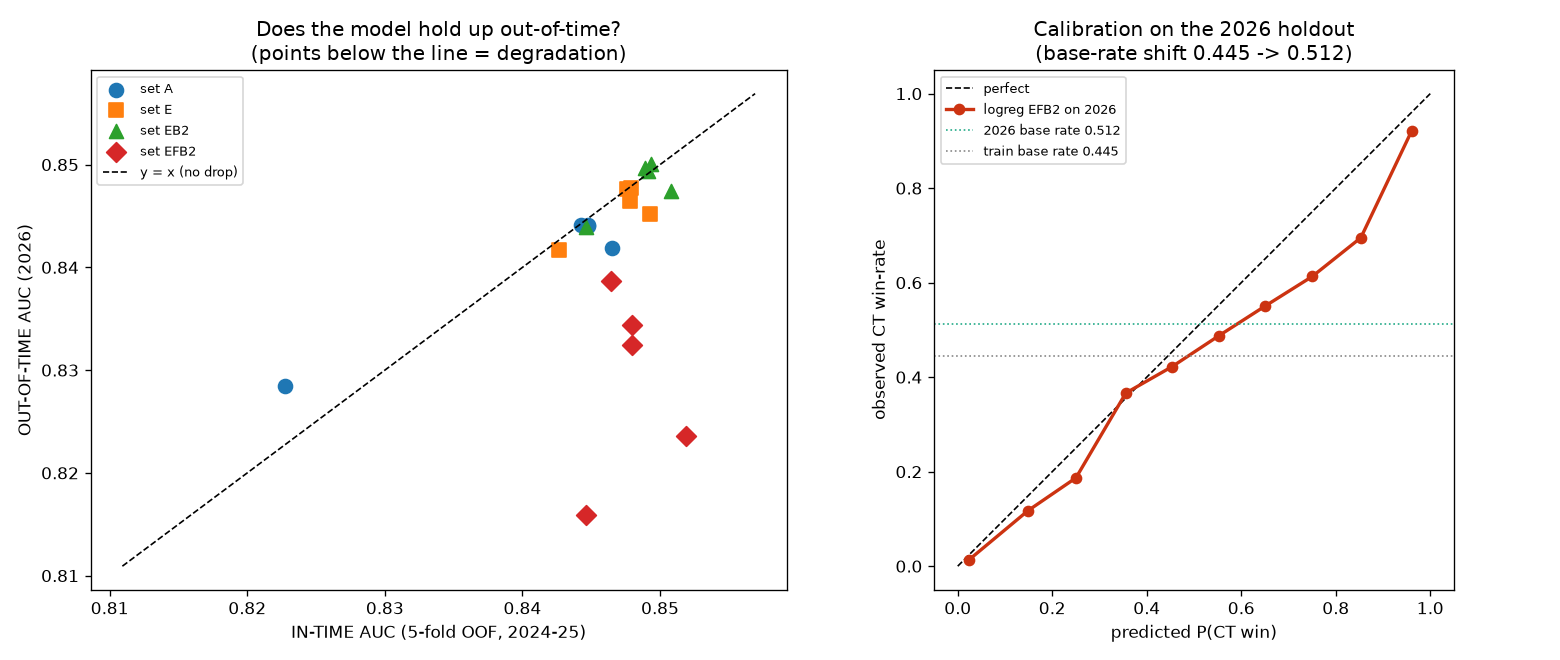
\includegraphics[width=\textwidth]{holdout_2026.png}
\caption{\textbf{Left:} in-time vs.\ out-of-time AUC. Points below the dashed line degraded.
Sets A/E/EB2 (no firepower) sit on the line --- they transfer. Every EFB2 point (red diamonds,
with firepower) falls well below it. \textbf{Right:} calibration of the best in-sample model
(logreg EFB2) on the holdout. It now sits systematically \emph{below} the diagonal:
over-confident in the CTs across the whole range (intercept $-0.36$), even though the true 2026
base rate ($0.512$) is \emph{higher} than training ($0.445$).}
\label{fig:holdout}
\end{figure}

\paragraph{The demo-derived pillars transfer essentially perfectly.}
Economy, Voronoi map control, tactical readiness and defuse-race geometry all generalise to a
new season, new game patches and substantially new rosters. Contested-AUC even \emph{improves}
out-of-time ($0.590 \to 0.64$--$0.65$). The non-firepower sets show only a benign base-rate
drift (calibration slope $\approx 1.0$, intercept $+0.11$ to $+0.13$) --- the expected
consequence of the $0.445 \to 0.512$ shift in CT win rate, and trivially correctable with a
single intercept adjustment.

\paragraph{But the best in-sample model becomes the worst out-of-time.}
Logistic EFB2 --- the study's best cross-validated model --- loses $0.0283$ AUC. Calibration
breaks with it: ECE $0.016 \to 0.071$, calibration intercept $\mathbf{-0.36}$. The right panel
of Fig.~\ref{fig:holdout} shows the damage: the reliability curve is dragged below the diagonal
across the entire range. The probabilities become untrustworthy, which for a live product is
the more serious of the two failures --- a model that is merely less accurate degrades
gracefully, whereas a model that is confidently wrong misinforms.

\paragraph{Diagnosis: a data-coverage failure, not a signal failure.}
Figure~\ref{fig:datagap} is the diagnosis. In 2026, \textbf{$\approx 30\,\%$ of players have no
entry in the HLTV skill database} --- rookies, stand-ins, and players who have not yet
accumulated a season of Tier-1 statistics --- and their contribution to the team skill-sum
silently becomes zero. The feature, tightly clustered at a mean of $5.28$ at 5-v-5 in training
(all five players known), collapses to a mean of $3.66$ on the holdout with a long tail toward
zero: \textbf{11.8\,\% of 2026 5-v-5 snapshots have a team skill-sum below 3, versus $0.0\,\%$
in training.}

\textbf{The same feature means something different in 2026.} And --- this is the cruel part ---
because it is a \emph{sum over alive players} (Sect.~\ref{sec:firepower}), a degraded value is
indistinguishable from a legitimate one: ``skill-sum 3'' means \emph{three good players alive}
in training and can mean \emph{five players, two of whom are unknown} in 2026. The model reads
the corrupted input as a real, familiar game state and mispredicts with confidence. That is why
the failure is silent, and why it damages calibration rather than merely accuracy.

\begin{figure}[H]
\centering
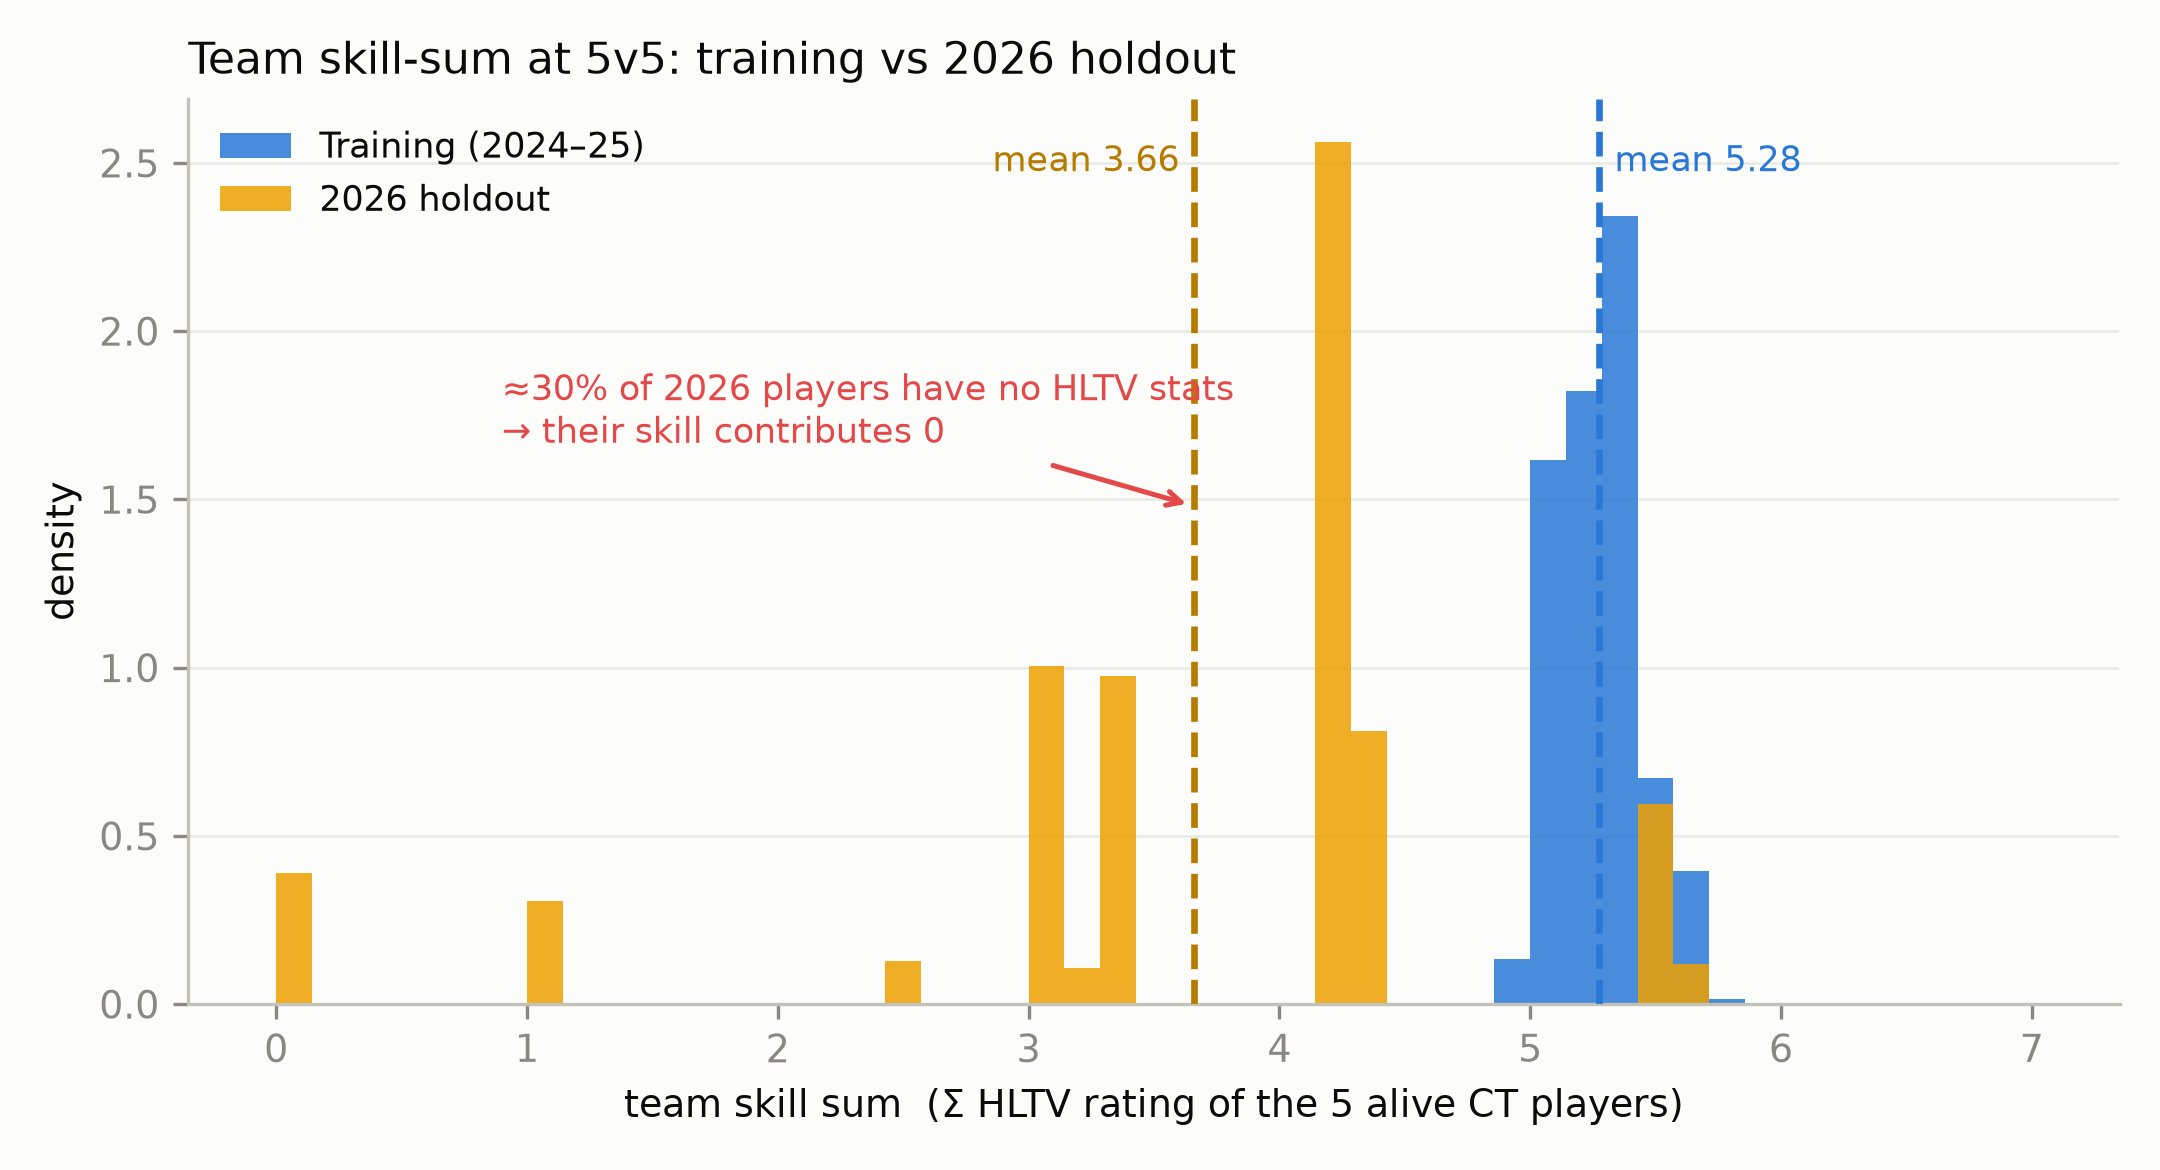
\includegraphics[width=0.95\textwidth]{F4_datagap.png}
\caption{Why firepower fails out-of-time. The team skill-sum at 5-v-5, tightly clustered in
training (mean $5.28$; all five players known), collapses on the 2026 holdout (mean $3.66$)
because $\approx 30\,\%$ of players have no database entry and silently contribute zero.}
\label{fig:datagap}
\end{figure}

\paragraph{The lesson.}
Pillars 1--3 are computed \emph{from the observation itself} and are therefore always available
at inference time. Pillar~4 is a \emph{prior sourced from outside the observation}, and
therefore carries an \textbf{inference-time data dependency}: at deployment it needs an external
database, indexed by an era which --- by definition --- is the era you have least data for. When
that database lags, the feature does not merely stop helping. \textbf{It actively harms the
model, and it does so silently.}

Cross-validation cannot see this. Every fold is drawn from the same era, in which the database is
complete; the feature is fully populated in both halves of every split. \emph{The failure is
invisible by construction to the standard protocol.} We therefore argue that any model
incorporating externally-sourced priors requires an out-of-time gate, and that its production
configuration should be chosen on out-of-time evidence rather than cross-validated evidence.

\textbf{Ours is EB2 --- with no firepower at all --- even though cross-validation ranked EFB2
first.}

\todo{The 2026 skill data does exist and is being collected. We will report a second,
\emph{separately disclosed} evaluation (the holdout above was touch-once; any re-run must be
declared as such) with (a) same-era 2026 statistics and (b) a leak-free \emph{lagged} prior using
the previous season's statistics. Note that (a) is itself mildly leaky --- a player's 2026 rating
is computed partly from the very matches being predicted, and would not exist at live inference
time --- so (b) is the deployment-realistic construction and the one that should headline.}

% =====================================================================
\section{Chronology: how we actually got here}
\label{sec:chronology}

Papers present findings in logical order; research does not happen in that order. This section
records what we built, in what order, and what each step taught us --- partly for honesty, partly
because the sequence contains most of the transferable engineering lessons.

\begin{enumerate}
  \item \textbf{Pipeline and the economy baseline.} Parse, validate, assemble, reproduce the
    literature baseline (AUC $0.8465$). Three silent parsing bugs surfaced here
    (Sect.~\ref{sec:pitfalls}); the halftime-swap bug in particular would have quietly capped
    everything downstream.

  \item \textbf{Regularisation before features.} Our first boosters ran at depth 6 and overfit.
    Fixing this was worth $+0.007$ AUC --- more than any feature pillar. Had we run the pillar
    ablations first, we would have measured every pillar against a noisy baseline and plausibly
    concluded that none of them worked.

  \item \textbf{Map control v1: Voronoi.} The football transfer. It worked ($+0.0025$), and we
    briefly believed spatial features were straightforwardly valuable.

  \item \textbf{Map control v2: the grey model.} We built the physically faithful version ---
    LOS, FOV, smoke occlusion, a $3060\times3060$ visibility matrix --- expecting it to beat
    Voronoi comfortably. \textbf{It lost.} This was the most surprising result of the project and
    we spent considerable time looking for a bug before accepting it was real.

  \item \textbf{Map control v3: territory.} The diagnosis (instantaneous control \emph{flickers})
    suggested the fix (memory). Territory recovered the loss but did not beat Voronoi, and is
    largely redundant with it. We kept Voronoi. Net result: a negative finding that we think is
    the most intellectually interesting thing in the paper (Sect.~\ref{sec:mapcontrol}).

  \item \textbf{Bomb pillar.} Three features built; one (the defuse race) is the best feature in
    the study, two (bomb-local control, dropped-bomb scramble) are worthless. We report all three
    (Sect.~\ref{sec:bomb}).

  \item \textbf{Firepower v1, and the \#1-ranked feature that meant nothing.} Permutation
    importance ranked team-rating-difference first of 68. The SHAP dependence plot
    (Fig.~\ref{fig:shapfirepower}) showed it was counting players. A lesson in not trusting an
    importance ranking on collinear inputs.

  \item \textbf{Firepower v2.} Rebuilt side-aware with situational gates to break the confound.
    Helps the linear model, hurts the trees, and --- because it kept the sums --- does not actually
    break the confound.

  \item \textbf{Deep models on GPU.} TCN, Transformer, GAT. All tie with logistic regression once
    the CIs are computed at the match level. The temptation to report the raw point estimates
    without match-level CIs was real, and would have produced a much more exciting and completely
    false paper.

  \item \textbf{The out-of-time holdout.} Run once, at the end. It inverted the ranking: our best
    model became our worst, and the pillar we had spent the most effort on turned out to be the one
    that cannot be deployed. Everything in Sect.~\ref{sec:holdout} follows.
\end{enumerate}

The through-line: \textbf{four of the ten steps above are negative results, and they carry more
information than the positive ones.}

% =====================================================================
\section{Discussion}
\label{sec:discussion}

\paragraph{Report contested-AUC.}
Pooled AUC on a per-second win-probability model is close to a measure of how often the game is
lopsided. Future Counter-Strike win-probability work should report performance on the even-round
subset, where all current models sit near chance and where improvement actually matters. We would
go further: a model that improved contested-AUC from $0.58$ to $0.62$ while \emph{losing} a point
of pooled AUC would be the more valuable model --- and the current convention would reject it.

\paragraph{Stability beats fidelity.}
The grey-vs-territory result suggests a general principle for tracking data: when the target is a
\emph{future} outcome, a representation's \emph{temporal stability} can matter more than its
instantaneous correctness. Practitioners building vision- or reachability-based control surfaces
should test a memory-augmented variant before concluding that control ``does not help''.

\paragraph{Physically-derived features beat learned ones at this scale.}
The defuse-race margin --- three quantities and a subtraction --- outperformed everything the deep
models discovered on their own from the same underlying distances. Figures~\ref{fig:shapdist} and
\ref{fig:shapdefuse} are the same geometry under two encodings; only one makes the feasibility
boundary learnable. With $\approx 5$k rounds, encoding known physics is a better use of capacity
than learning it.

\paragraph{Beware the external prior.}
This is the finding we most want to travel. A ``skill prior'', ``player form'', ``team strength''
or any feature joined from an outside table introduces a dependency that cross-validation is
structurally blind to. Such a feature should be (a) gated by an out-of-time evaluation,
(b) constructed as a \emph{lag} --- using only information that existed before the event being
predicted --- and (c) monitored for \emph{coverage} in production, with an explicit fallback (a
per-capita encoding, an imputed league average, or dropping the pillar) for when coverage drops.
None of these is exotic. What is easy to miss is that \emph{nothing in the standard protocol tells
you that you need them}.

% =====================================================================
\section{Limitations}
\label{sec:limitations}

\begin{enumerate}
  \item \textbf{Single map.} All results are \textit{de\_inferno}. Spatial features are
    map-specific by construction; multi-map generalisation is untested.
  \item \textbf{Scale.} 220 matches, $\approx 4{,}900$ rounds. The deep-model dead heat is a
    statement about this regime and should not be read as a general claim.
  \item \textbf{Firepower leakage.} Same-era player ratings are partly computed from the matches
    being predicted, and would not exist at live inference time. The lagged-prior variant (in
    progress) is the clean construction.
  \item \textbf{Firepower count confound.} The summed-rating feature is approximately a
    player-count proxy ($r = 0.987$; Fig.~\ref{fig:shapfirepower}). We report rather than repair
    it, since Sect.~\ref{sec:holdout} shows the binding constraint is data coverage, not encoding.
  \item \textbf{Irreducible ceiling.} Contested rounds sit near $0.58$ for \emph{every} model
    tested. Some of this is genuine aleatoric randomness --- a 5-v-5 on equal buys really is close
    to a coin flip, and it should be. How much is irreducible and how much is headroom is unknown,
    and is the most important open question this work leaves.
  \item \textbf{Deep-model holdout.} The deep models were not re-evaluated out-of-time.
    \todo{decide whether to run this on EB2 --- they inherit the same firepower dependency, so the
    interesting question is only whether they degrade \emph{more} than the classical models}
  \item \textbf{Single holdout era.} One out-of-time window (2026). The failure mode we identify is
    general, but its \emph{magnitude} here is a single observation.
\end{enumerate}

% =====================================================================
\section{Conclusion}
\label{sec:conclusion}

We built a per-second win-probability model for Counter-Strike~2 and used it to interrogate three
conventions of the field.

Pooled AUC flatters: restricted to even rounds, every model is near a coin flip, and we propose
contested-AUC as the honest metric. Physical fidelity does not imply predictiveness: the most
realistic map-control model is the least useful until it is given memory. And cross-validation is
not a deployment test: our best cross-validated model became our worst out-of-time, because one
pillar depended on a database the future does not yet have --- a failure mode that grouped folds
cannot expose.

The features that \emph{did} transfer --- economy, Voronoi map control, and a three-term
defuse-race inequality --- are the ones computed directly from the game itself.

% =====================================================================
\section*{Acknowledgements}
\todo{PARCC allocation acknowledgement --- required by their terms of use.}

\bibliographystyle{plain}
\bibliography{refs}

% =====================================================================
\appendix

\section{Reproducibility notes}
\label{app:repro}

\paragraph{Parsing.} \texttt{awpy}~v2.0.2, tickrate forced to 64.

\paragraph{Splits.} 5-fold \texttt{GroupKFold} keyed on \texttt{match\_id}. The 2026 holdout lives
in a physically separate directory tree and is assembled through a separate code path, so no glob
over the training directories can sweep it in.

\paragraph{Bootstrap.} $B = 500$ resamples of \emph{matches} (with replacement), recomputing all
metrics on fixed out-of-fold predictions. For the holdout, the 27 test matches are the resampling
unit.

\paragraph{Compute.} Classical models train on a laptop CPU in minutes. The three deep models were
trained on an NVIDIA B200 (PARCC Betty). \todo{exact wall-clock and epochs}

\section{Full metric battery}
\label{app:metrics}
\todo{Table of every model $\times$ feature set with log-loss, Brier, ECE, BSS, reliability /
resolution / uncertainty, adaptive ECE, KS-cal, calibration slope and intercept, and contested-AUC,
all with bootstrap CIs. These exist in \texttt{outputs/} already --- this is a formatting job, not an
experiment.}

\section{Supplementary figures}
\label{app:extra}

\todo{Candidates already rendered in \texttt{outputs/figures/}, not yet placed:
\texttt{logistic\_coefficients.png} (the fitted linear model, directly interpretable);
\texttt{plant\_spots.png} (where the bomb actually gets planted on Inferno --- motivates the
site-control zones); \texttt{shap\_beeswarm\_ET\_xgb.png} (global feature attribution);
\texttt{mapcontrol\_snapshots\_faze-vs-g2\_r5.png}; the reliability-per-model grid; and the
remaining win-probability case studies.}

\end{document}
